\chapter{INTRODUCTION}
\label{chap:intro}
\section{Motivation}
One of the problem for visually impaired individuals is that they are mostly been cheated during money transactions such as they are not able to distinguish between different currency and also they face difficulty in taking their medicines as most of the medicine tablets are in same in size hence they face difficulty in identifying that which medicine they need to take in what quantity and at what time and for this thing they always need to depend on somebody else so taking their problem into account. So, an idea to develop an software based personal assistance that will guide them when they will face these two problems in future.
\section{Objective of the Project}
The main objective of this project work is to help the visually impaired individual (blind person) by protecting them from getting cheated in terms of money transaction and also to reduce their dependence on other people for taking right medicines in right quantity at right time. To fill this main objective, identified the following objectives for the proposed work.\\
\noindent{\bf (a) Machine learning model for currency detection.}\\
\noindent{\bf (b) Algorithm to guide them with proper medicine name with prescribed doses using Image processing and OCR  .}
\newpage
\chapter{SOFTWARE DESCRIPTION}
\section{Image Processing}
\noindent Image processing is a method to perform some operations on an image, in order to get an enhanced image or to extract some useful information from it. It is a type of signal processing in which input is an image and output may be image or characteristics/features associated with that image.\\It involves the operations required prior to data analysis and information extraction. Here image pixels are extracted then cropping, scaling, conversion of image into grey level,finding counters is done. In Figure 2.1. (a) and Figure 2.1. (b)  thresholding and adjustment of brightness and contrast is shown respectively using image processing.\citeauthor{9020106}\\
\begin{figure}[h!]
	\centering
	\includegraphics[]{}
	\subfigure[]{\label{fig:a}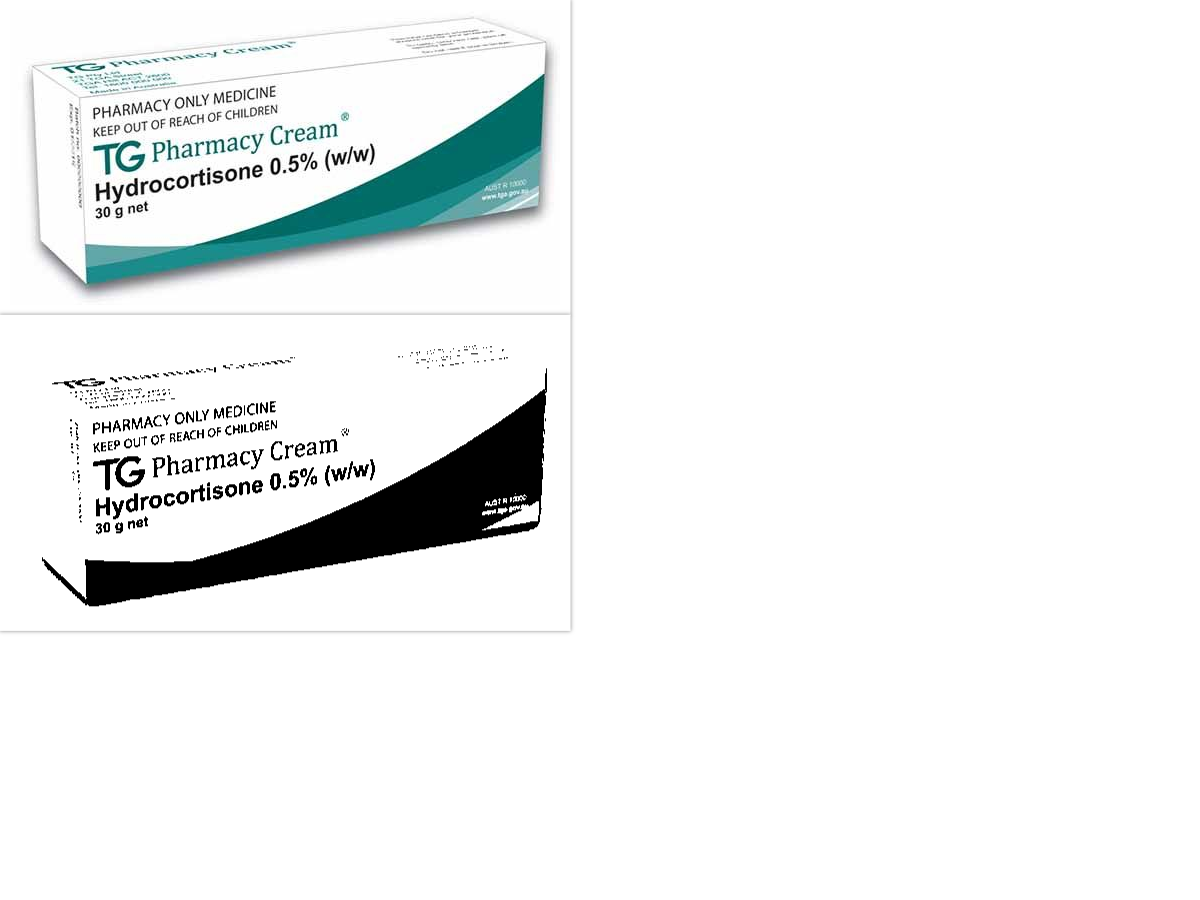
\includegraphics[width=60mm]{CHAPTERS/med.png}}
	\subfigure[]{\label{fig:b}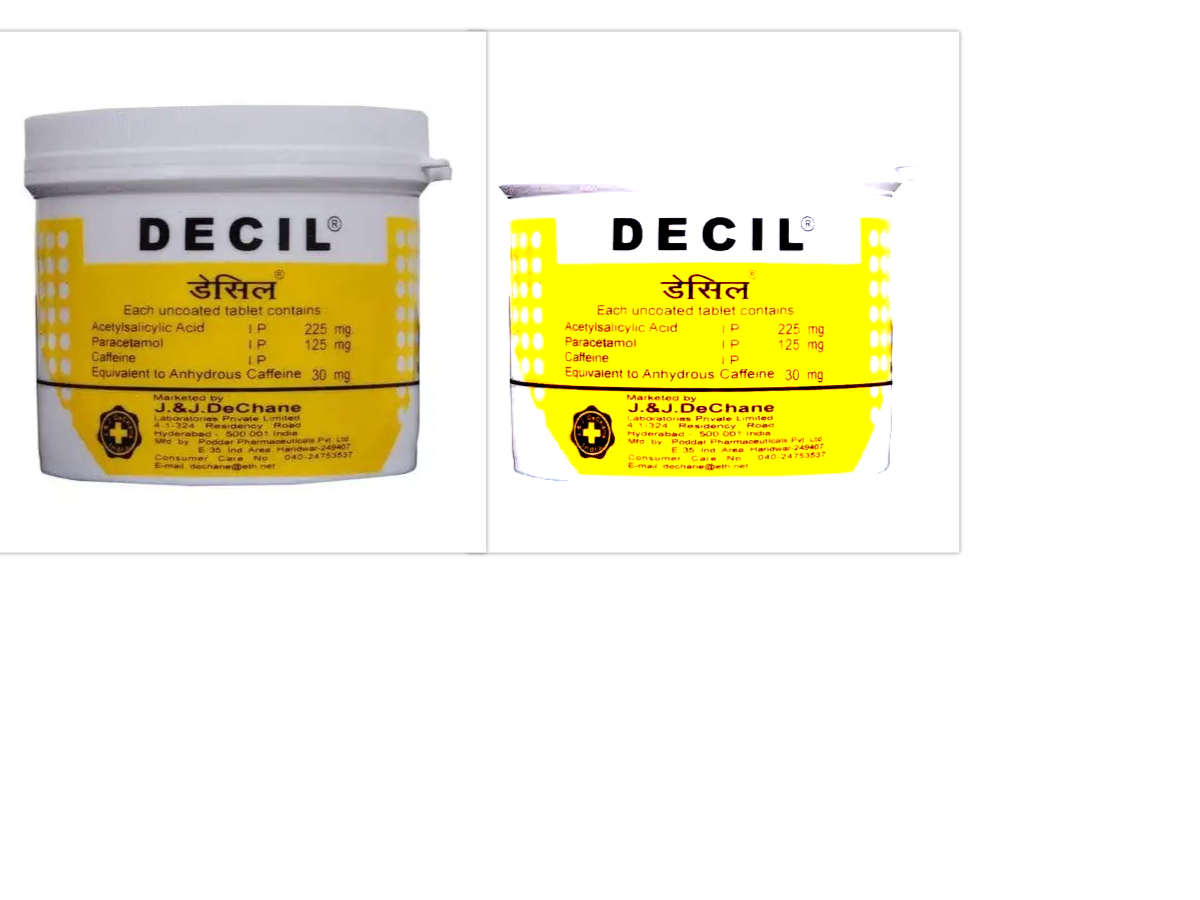
\includegraphics[width=60mm]{CHAPTERS/dec (1).png}}
	\caption{(a) Thresholding effect (b) Brightness and Contrast adjustment effect}
\end{figure}
\textbf{Operations used under this project}
\begin{itemize}
    \item Thresholding of an image
    \item Brightness and contrast adjustment
    \item Image enhancement
\end{itemize}
\newpage
\section{OpenCV}
\noindent OpenCV (Open Source Computer Vision Library) is an open source library of programming functions mainly aimed at real-time computer vision.It is library to all for image processing applications. CV2 library is used in this project for the manipulation of image for both currency and medicine detection. \citeauthor{9020105}\\Converting an image RGB to gray scale using OpenCV function CV2.RGB2GRAY in Spyder IDE using python CV2 module is shown below in both Figure 2.2. (a) and Figure 2.2. (b) as a example of hundred rupee note.\\
\textbf{Operations used under this project}
\begin{itemize}
    \item RGB to Gray Scale conversion
    \item Cropping of an image
    \item Capturing the image
    \item Resizing the image
\end{itemize}
\begin{figure}[h!]
	\centering
	\includegraphics[]{}
	\subfigure[]{\label{fig:a}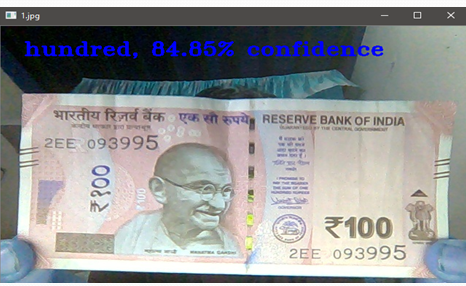
\includegraphics[width=60mm]{CHAPTERS/x9.png}}
	\subfigure[]{\label{fig:b}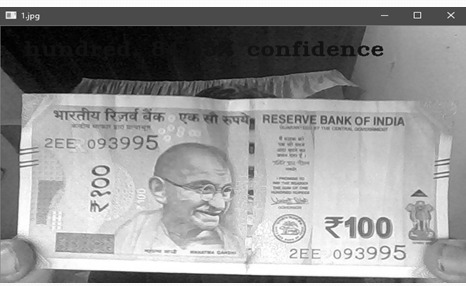
\includegraphics[width=60mm]{CHAPTERS/gray.jpg}}
	\caption{(a) Hundred rupees note image captured using OpenCV (b) Gray scale image of hundred rupees note using OpenCV}
\end{figure}
\section{OCR}
\noindent OCR is used to recognize the the characters from the captured image and convert it into textual information as shown below in Figure 2.3. where input is an image and output is a text. The basic process of OCR involves recognize the text of a image and translating the characters into code that can be used for data processing.
OCR is used here in this project as text recognition.\citeauthor{9020104}\\
\textbf{Operations used under this project}
\begin{itemize}
    \item Pattern recognition : It is used to discriminate the fonts and formats by compare, and recognize.
    \item Feature detection : It is used to discriminate the letters and numbers by number of angled lines, crossed lines or curves in a character.
\end{itemize}
\begin{figure}[h!]
	\centering
	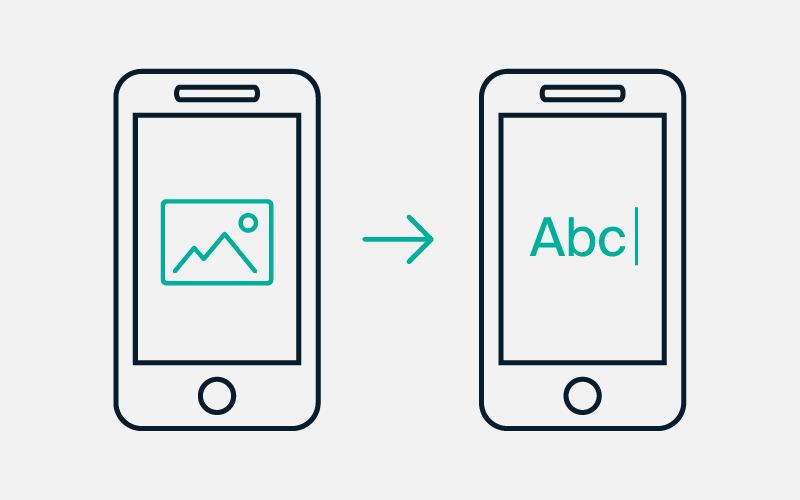
\includegraphics[width=80mm]{CHAPTERS/ocr.png}
	\caption{OCR}
\end{figure}
\noindent
\textbf{Tools were used under this project for OCR}
\begin{itemize}
    \item Tesseract Engine : Tesseract is an optical character recognition for which set-up of an engine has to be done earlier and its an open source to all and tesseract uses apache server.\citeauthor{9020103}
\end{itemize}
\section{Machine Learning}
\noindent Machine learning (ML) is the study of computer algorithms that improve automatically through experience.It is seen as a subset of artificial intelligence. Machine learning algorithms build a mathematical model based on sample data, known as "training data", in order to make predictions or decisions without being explicitly programmed to do so. In this project Machine Learning is Used for creating the dataset and train the model for the currency detection part in the project.\citeauthor{9020108}\\
\newpage
\textbf{Tools used under this project for machine learning}
\begin{itemize}
    \item Spyder IDE
    \item Anaconda
    \item Google Colab
\end{itemize}
\section{Django}
\noindent Django is a free and open source, full-stack web application framework, written in Python and widely used for web app development with administration GUI. Django is used in this project to give the user interface. Django upload our complete project files onto its own server.\citeauthor{four}\\\\ \\
\noindent
\textbf{Tools used under this project for Django}
\begin{itemize}
    \item Virtual Studio Code : Used to write the code and commit the changes to the GitHub
    \item Anaconda prompt : Used to run the command for uploading files to the Django server, installing the required libraries and virtual environment setup for specific tasks.
    \item Google Chrome : Used to open the interface and development tools to edit the designs while making the interface.
\end{itemize}
\\\\
\section{Talkback and Voiceover}
\noindent Features of both talkback and voiceover  accessibilities in both android and iOS is shown above in Figure 2.4. (a) and Figure 2.4. (b).\\
\begin{itemize}
     \item Talkback and voiceover is the accessibility service given by android and iOS respectively for Blind person.
\end{itemize}
\begin{figure}[h!]
	\centering
	\includegraphics[]{}
	\subfigure[]{\label{fig:a}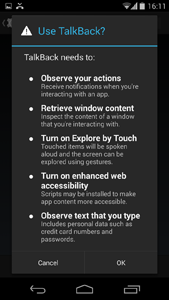
\includegraphics[width=50mm]{CHAPTERS/talkback.png}}
	\subfigure[]{\label{fig:b}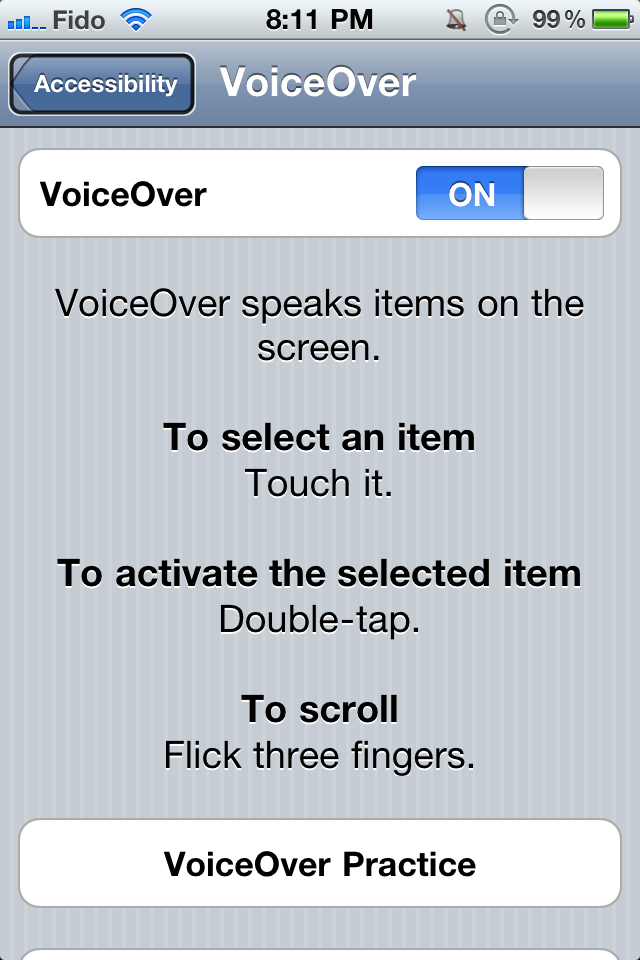
\includegraphics[width=58mm]{CHAPTERS/voiceover.png}}
	\caption{(a) Talkback feature in android (b) VoiceOver feature in iOS}
\end{figure}
\newpage
\noindent 
\begin{itemize}
 \item Talkback and voiceover provides spoken feedback as you navigate around the screen, by describing  your actions and informing you of notifications. It is a system application and comes pre-installed on most of the Android devices.
    \item By using these feature it is very easy for the blind person to operate mobile phone.\citeauthor{9020109}
\end{itemize}\\
\textbf{Steps to be followed for talkback by blind person:}
\begin{itemize}
    \item Press Volume up and Volume down keys for 3 second to turn on talkback  feature
    \item Click on medicine and currency web app
    \item Choose the file button
    \item Select the camera option among the all option and click the medicine or currency image
    \item Select the image by using done button at bottom right on the screen
    \item Press submit button
\end{itemize}

\chapter{CURRENCY DETECTION}
\section{Overview}
As mentioned in the problem statement currency detection in this report is one of the major problem faced by blind people in our society.To overcome that problem an innovative idea which is cheap and cost efficient. In this project mobile phone camera is used for getting the input, where the inputs are pictures of currency, and then with the help of web application which is build by using Django interface sends these pictures on to the Django server. \\ A currency dataset is created and trained by convolution neural network model through machine learning algorithms. Trained model is already uploaded on to the Django server and camera of the device will take the input image and compare it with the trained dataset.\\
If the image features matches with the dataset features then it will give a audio file (using TTS technology in python code) to the Django interface and then the user will get to now the currency. 
\begin{figure}[h!]
	\centering
	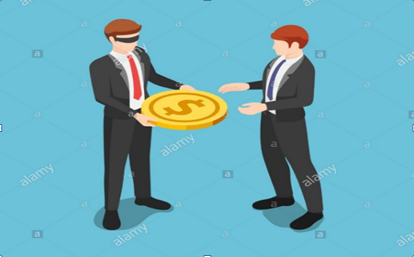
\includegraphics[width=80mm]{CHAPTERS/c1.PNG}
	\caption{Blind person struggling to detect currency}
\end{figure}
\newpage
\section{Block Diagram}
The Block Diagram of Currency Detection is shown in Figure 3.2.
\begin{figure}[h!]
    \centering
    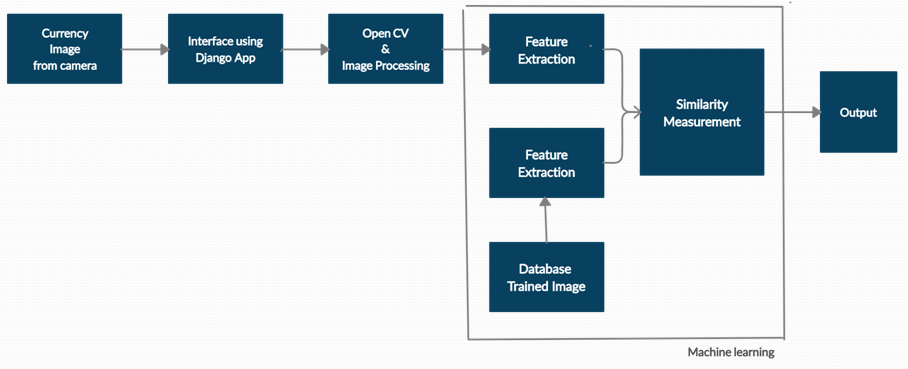
\includegraphics[width=0.9\textwidth]{CHAPTERS/c2.PNG}
    \caption{Block diagram}
\end{figure}
\section{Working}
Currency image is taken using the Mobile camera. Web application id created using Django interface and once the image is taken using the mobile phone then it is send to the local web server as an input. Image processing is used to extract necessary information. Open CV is used to threshold image, colour shifting, scanning and cropping, setting grey level, and to extract contours. On the other hand an dataset is created for different types currency like {\bf 10, 20, 50, 100, 200, 500} each having atleast 800 images. Then training of CNN model is done with logistic classification so that the model will extract the features of different currency available in database.\\
Further, the trained model is uploaded on to local server [Django server] where this model will take the input image and extract its features and if the features of the input image matches with the predefined dataset features,then it will give a audio file (using TTS) to the Django interface and tell the user for which currency he/she is facing trouble. \citeauthor{9020096}\\


\section{Methodology}
{\bf 1) Image acquisition:}\\ 
The image is captured through a simple digital Camera using the mobile phone.\\
{\bf 2) Image preprocessing:}\\ 
It involves the operations required prior to data analysis and information extraction. Here image pixels are extracted then cropping, scaling, conversion of image into grey level,finding counters is done.\\
{\bf 3) Gray scale conversion and edge detection:}\\ 
The acquired image is obtained as RGB image which is now converted into gray scale image as shown in Figure 3.3.  since it carries intensity information. This image is further processed and edges of gray scale images are detected.\\
\begin{figure}[h!]
	\centering
	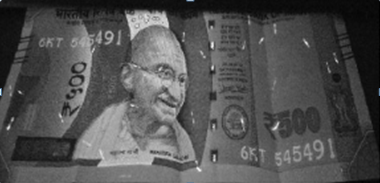
\includegraphics[width=80mm]{CHAPTERS/m1.PNG}
	\caption{Gray scale image}
\end{figure}
\noindent{\bf 4) Image segmentation:}\\
It’s the process of dividing image into multiple parts by cropping it. As it is shown in Figure 3.4. (a) in which the identification mark is segmented.\\ 
{\bf 5) Feature extraction:}\\ 
Now the features are extracted using edge based segmentation technique as shown in Figure 3.4. (b), Figure 3.5. (a),Figure 3.5. (b) \citeauthor{9020097}\\

\begin{figure}[h!]
	\centering
	\includegraphics[]{}
	\subfigure[]{\label{fig:a}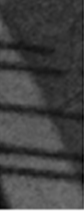
\includegraphics[width=20mm]{CHAPTERS/m2.PNG}}
	\subfigure[]{\label{fig:b}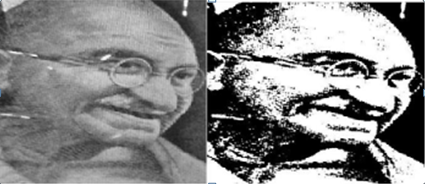
\includegraphics[width=70mm]{CHAPTERS/m3.PNG}}
	\caption{(a) Identification mark (b) Edge segmentation of Mahatma Gandhi portrait.}
\end{figure}
\newpage
\begin{figure}[h!]
	\centering
	\includegraphics[]{}
	\subfigure[]{\label{fig:a}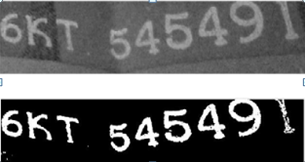
\includegraphics[width=60mm]{CHAPTERS/m4.PNG}}
	\subfigure[]{\label{fig:b}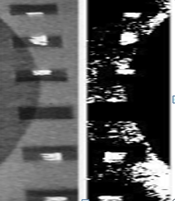
\includegraphics[width=40mm]{CHAPTERS/m5.PNG}}
	\caption{(a) Edge based segmentation of serial number(b)Edge based segmentation of security thread.}
\end{figure}
\vspace*{1cm}
\newline
\noindent{\bf 6)} Now the process of calculation of intensity of each extracted feature is done using {\bf CNN model}.If the calculated intensity of the input image is greater than the threshold of 75 percent of a particular currency,then it is classified as original note of that currency otherwise it is considered as a fake one.\\
{\bf 7)}The final decision depends upon the intensities of all extracted features.
\newpage
\noindent\textbf{CNN Model}\\

\noindent Started with an input image on which it will apply multiple different feature detectors which are also called as filters to create these feature maps and these feature maps together creates our convolution layer as shown in Figure 3.6. Then on the convolution layer {\bf RELU} is applied to remove the increased linearity in our image.\\
\begin{figure}[h!]
	\centering
	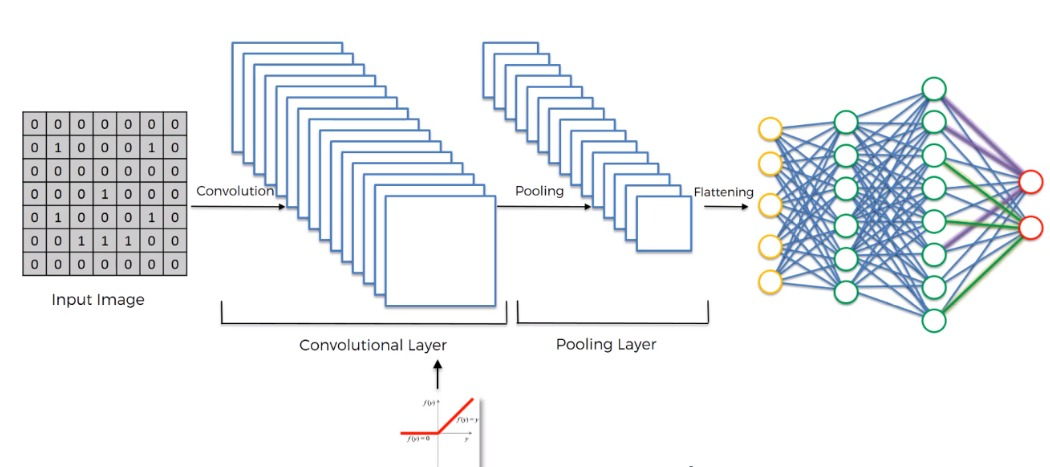
\includegraphics[width=1\textwidth]{CHAPTERS/m6.jpeg}
	\caption{CNN Model}
\end{figure}
\noindent Then pooling layer is applied to the convolution layer so that from every feature map it will create a pool feature map, so that it reduces the size of the image and also preserves its features. There are different types of pooling, here the {\bf MAX POOLING} technique is considered.Flattering took place where all the pooled images values are flatten into one array column of all the values.Now,this column is considered as an input for artificial neural network where two fully connected layers or the hidden layers are formed.These hidden layer are formed from neurons. Here all the features of the images are processed through the network and then the hidden or fully-connected layer performs voting based on different features towards different classes which where formed and then the probability will be determined using the softmax function. Softmax usually turns numbers to probability and based on the probability the correct class is identified.
\citeauthor{9020108}
\newpage
\noindent{\bf Data Acquisition}\\
\noindent The dataset is the most important part of a neural network-based project. It is very important to select a dataset that contains a variety of images. These images should be in different backgrounds or backdrops and preferably should images with different exposure and contrasts too.it is preferable to have a dataset of labelled images classified into different categories. The dataset with a higher number of images is preferred to train the neural network as it helps improve the generalization of the system.\\In this project dataset for six different currencies are made as shown in Figure 3.7. and each dataset of currency with approx {\bf 800 images} .\\\\
\begin{figure}[h!]
	\centering
	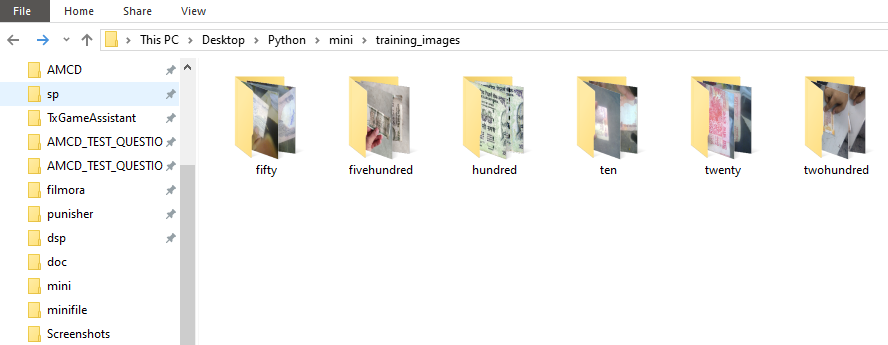
\includegraphics[width=100mm]{CHAPTERS/data2.PNG}
	\caption{Dataset for currency detection}
\end{figure}
\begin{figure}[h!]
	\centering
	\includegraphics[]{}
	\subfigure[]{\label{fig:a}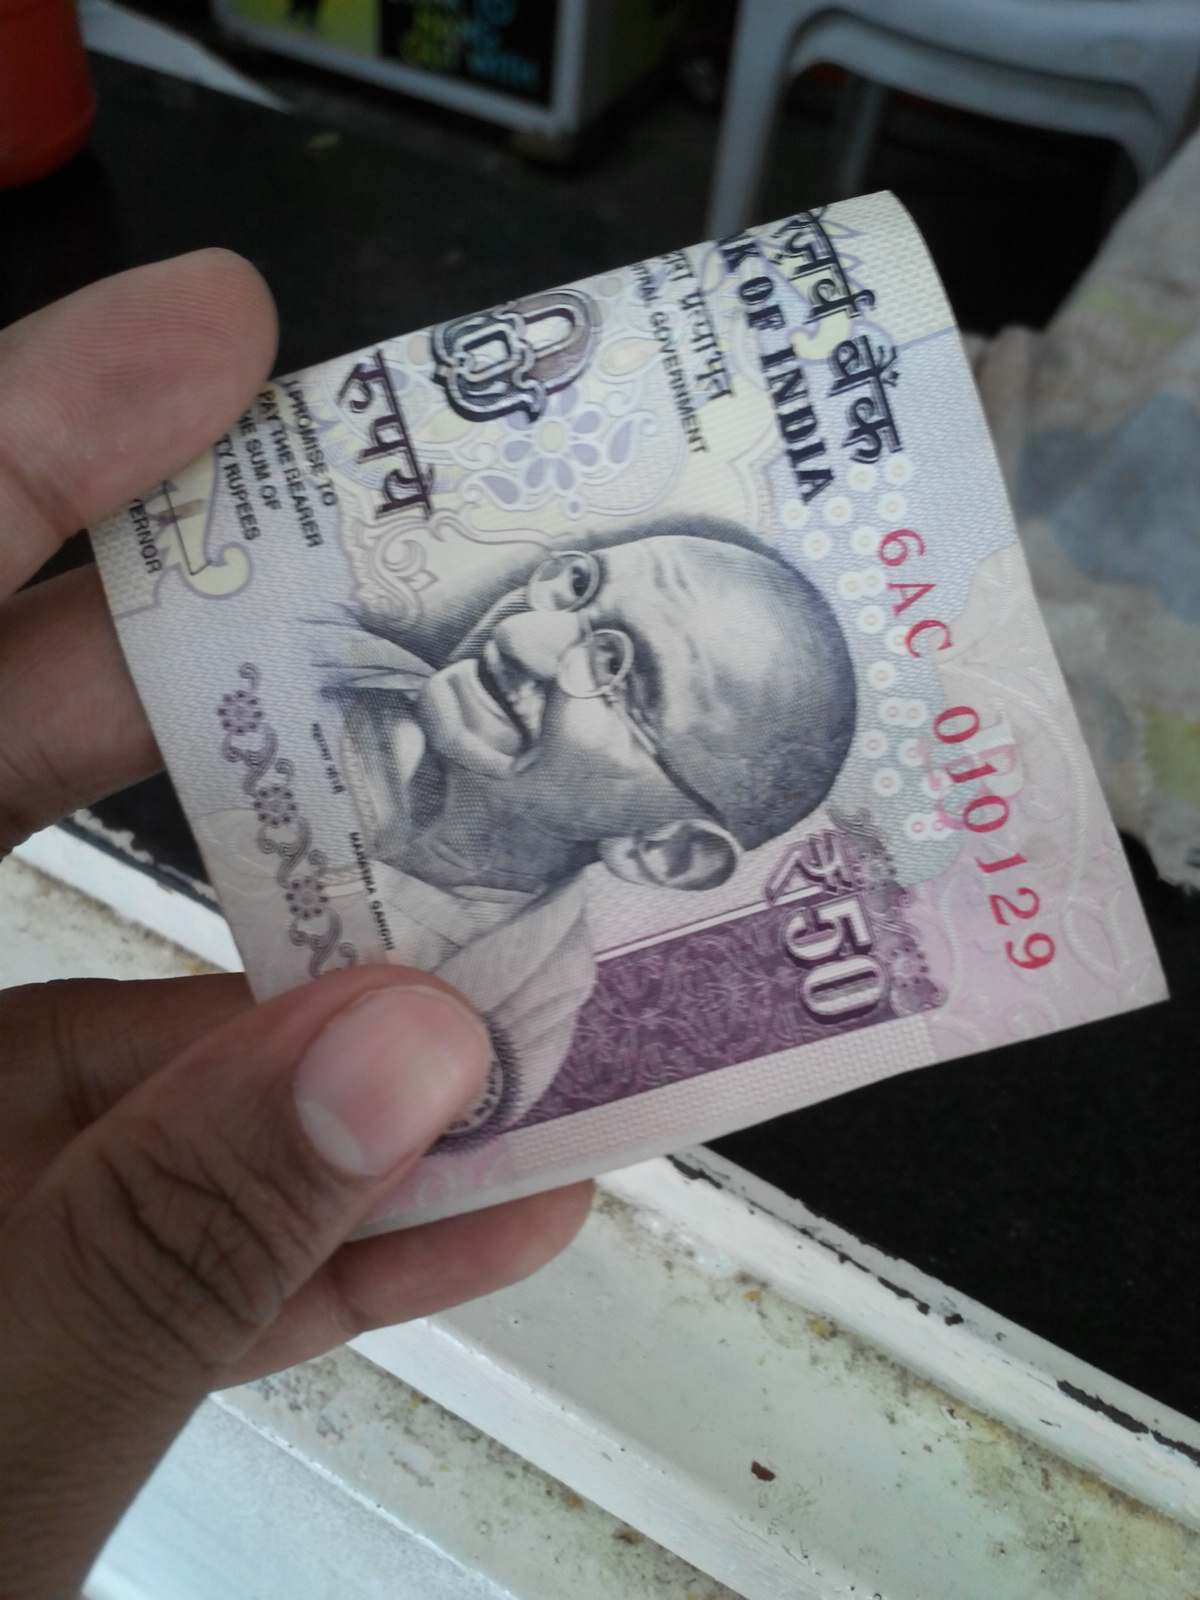
\includegraphics[width=60mm]{CHAPTERS/ff1.jpg}}
	\subfigure[]{\label{fig:b}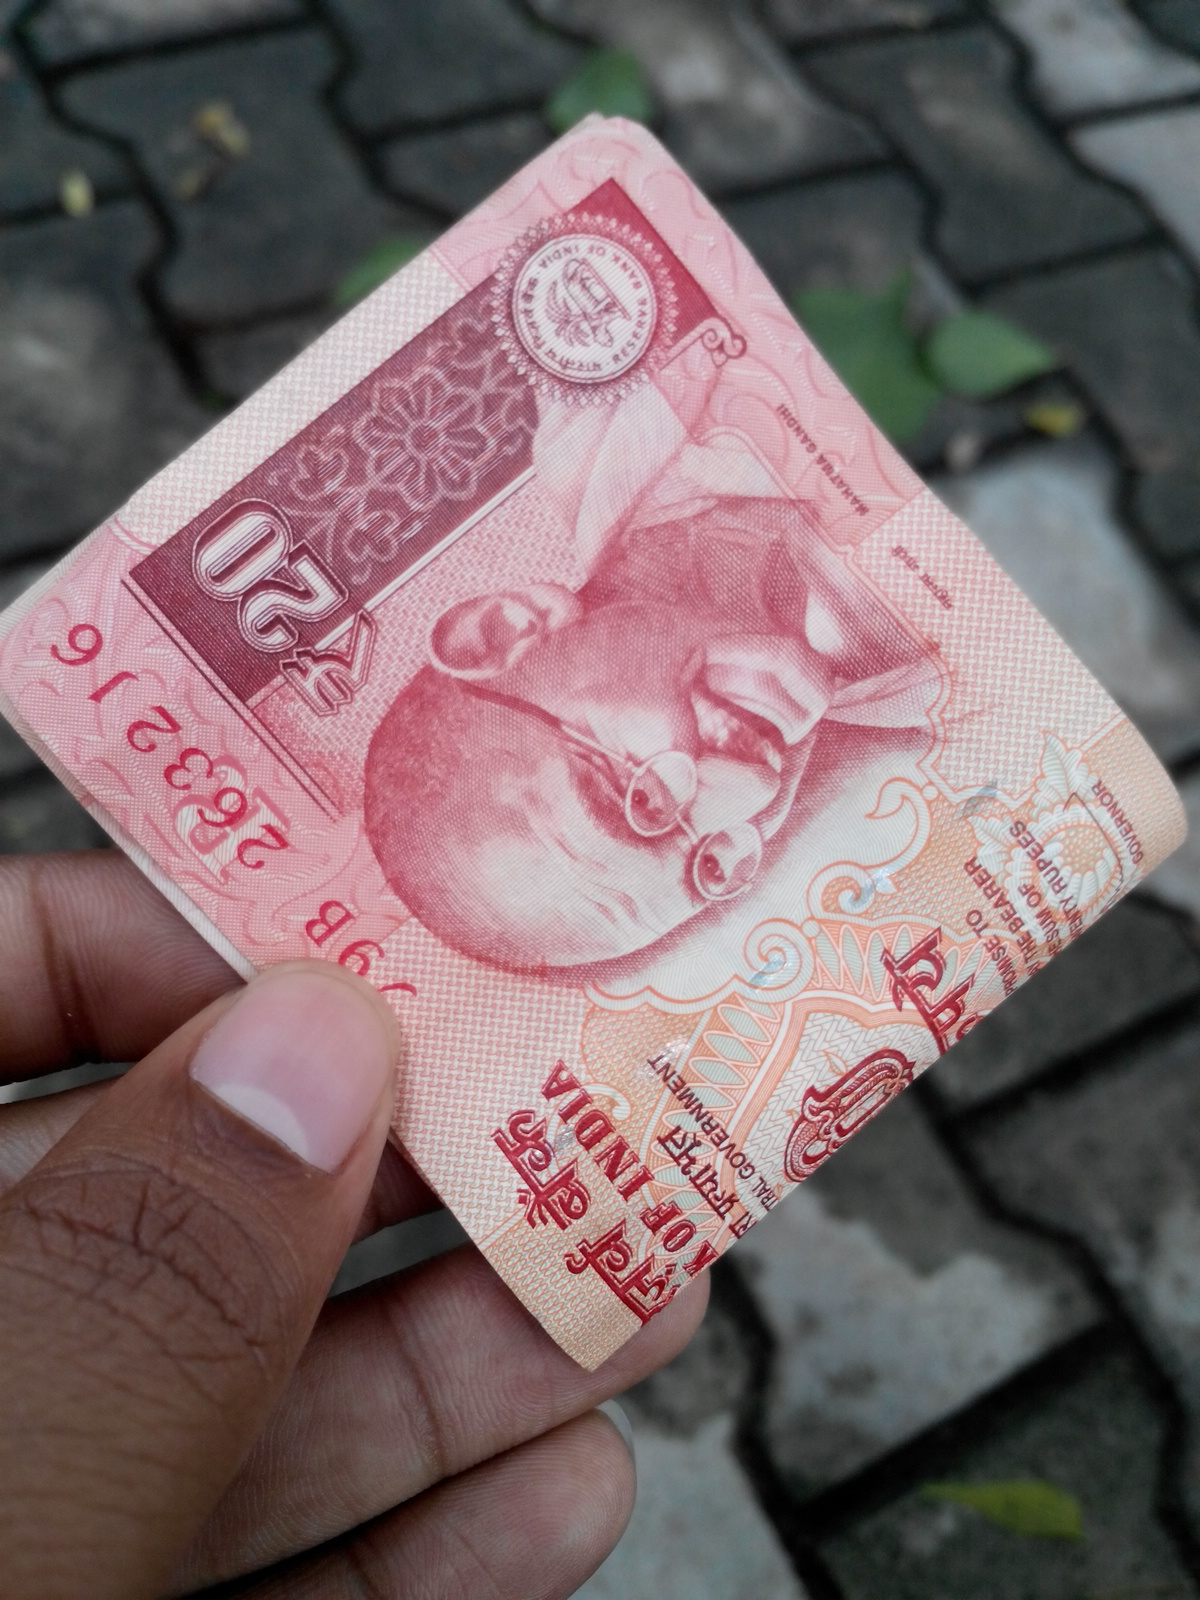
\includegraphics[width=60mm]{CHAPTERS/f4.jpg}}
	\caption{Dataset of currency image  taken in folded condition}
\end{figure}
\\\\
Dataset of each currency is created with the images of that currency in all conditions(poor light,bright light) and from all angles such that if a person will show the currency from any angle to the camera then the model is able to recognize the currency with good accuracy.\\\\
The below figure 3.8 shows the dataset of currencies taken in folded condition so that if a person try to recognize the currency in folded condition then the model will be able to determine the currency with high accuracy.\\\newpage
\begin{figure}[h!]
	\centering
	\includegraphics[]{}
	\subfigure[]{\label{fig:a}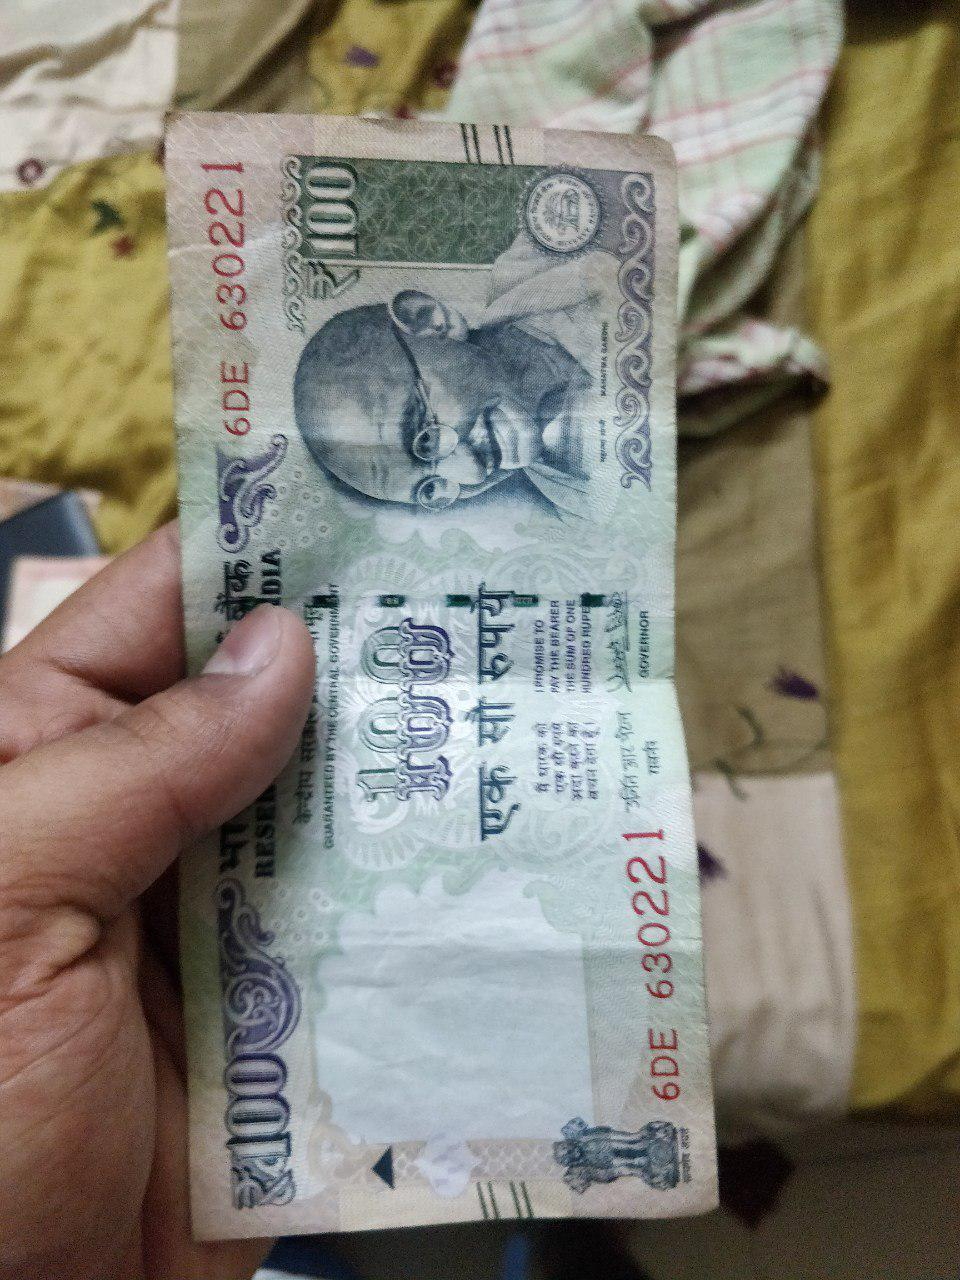
\includegraphics[width=60mm]{CHAPTERS/gd.jpg}}
	\subfigure[]{\label{fig:b}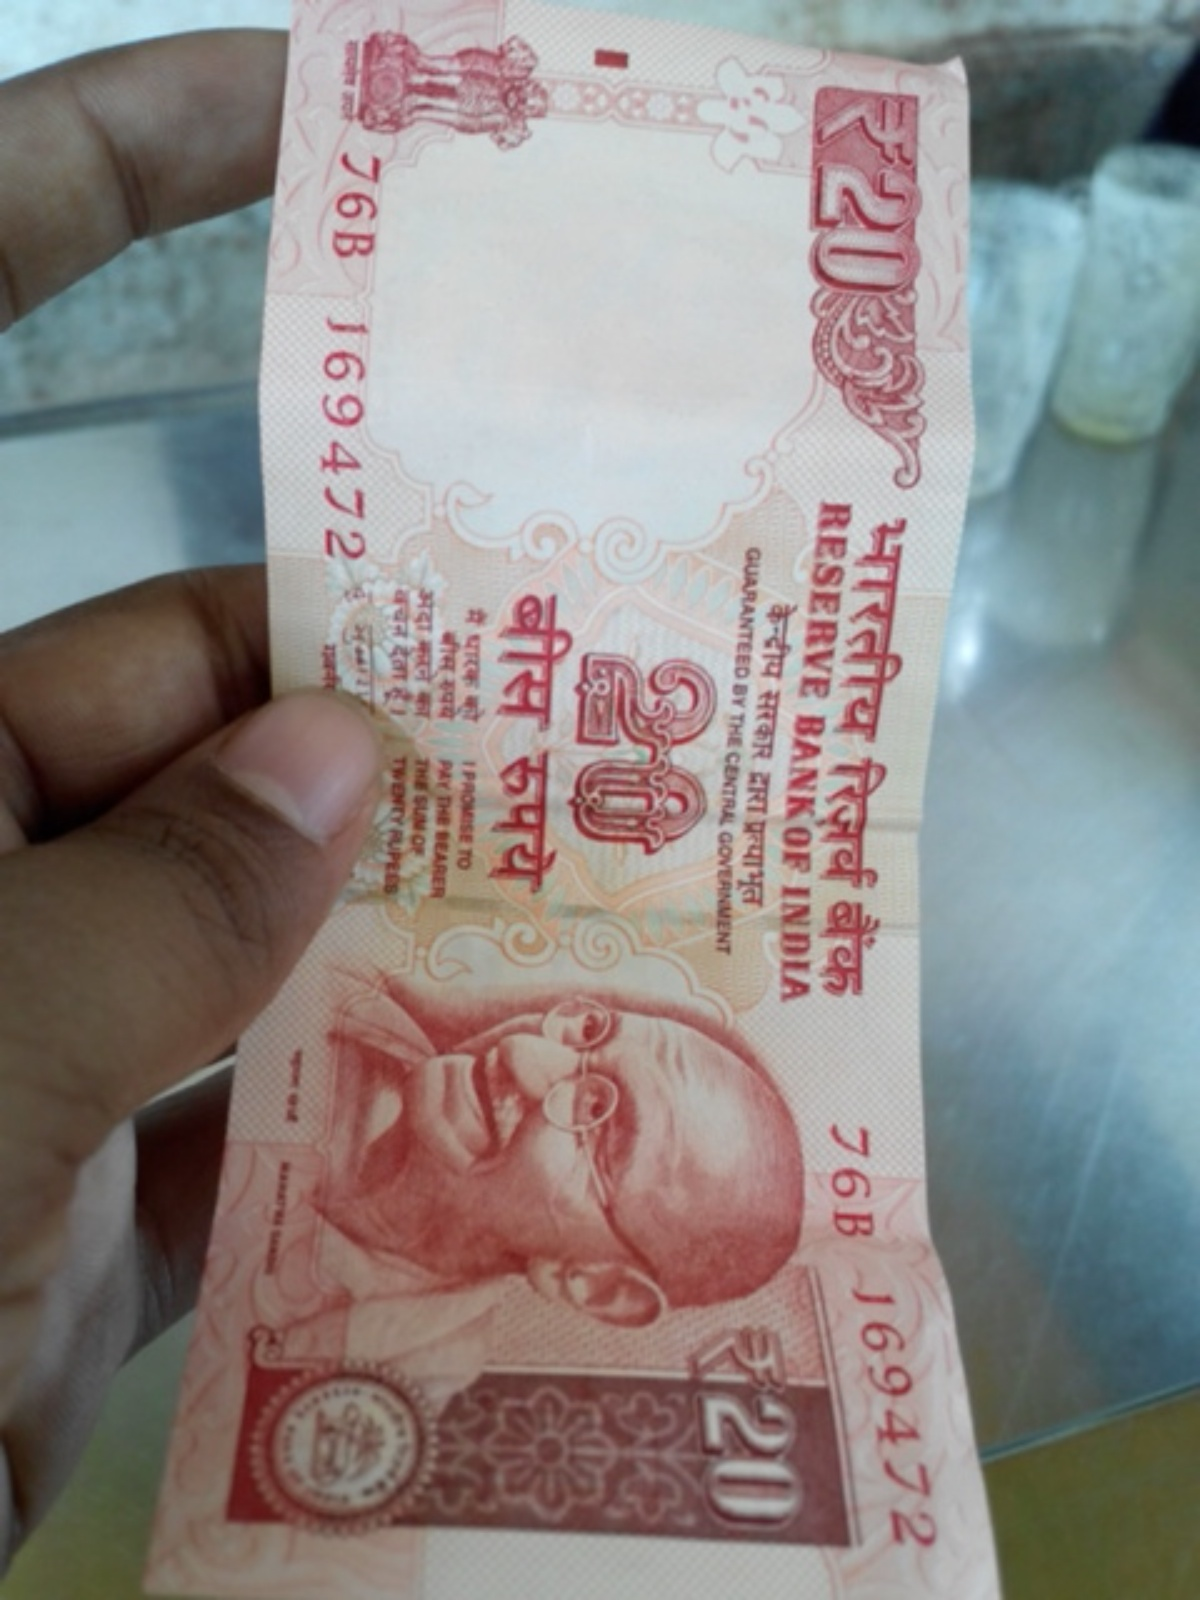
\includegraphics[width=60mm]{CHAPTERS/gd1.jpg}}
	\caption{Dataset of currency image taken from front side and in good light condition}
\end{figure}
\\
\noindent The above figure 3.9. shows the dataset of currencies taken from front position and in good lighting condition\\\newpage
\begin{figure}[h!]
	\centering
	\includegraphics[]{}
	\subfigure[]{\label{fig:a}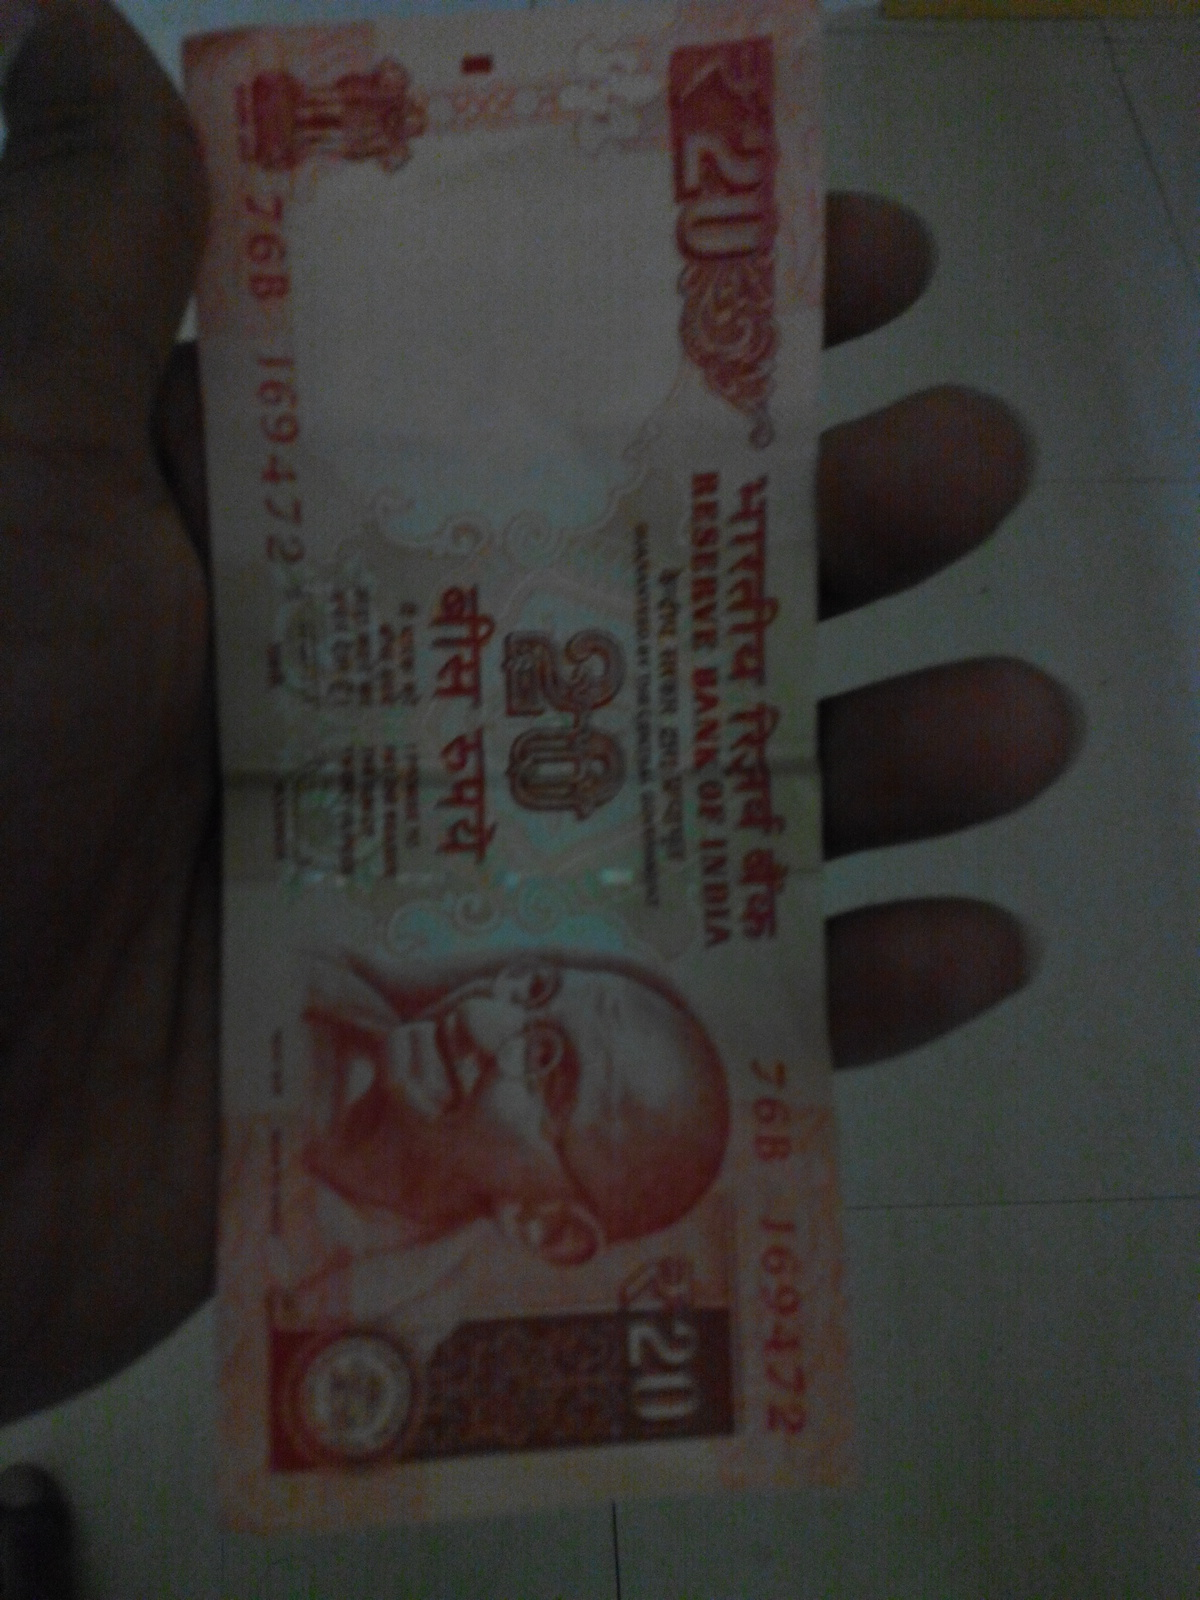
\includegraphics[width=50mm]{CHAPTERS/bd3.jpg}}
	\subfigure[]{\label{fig:b}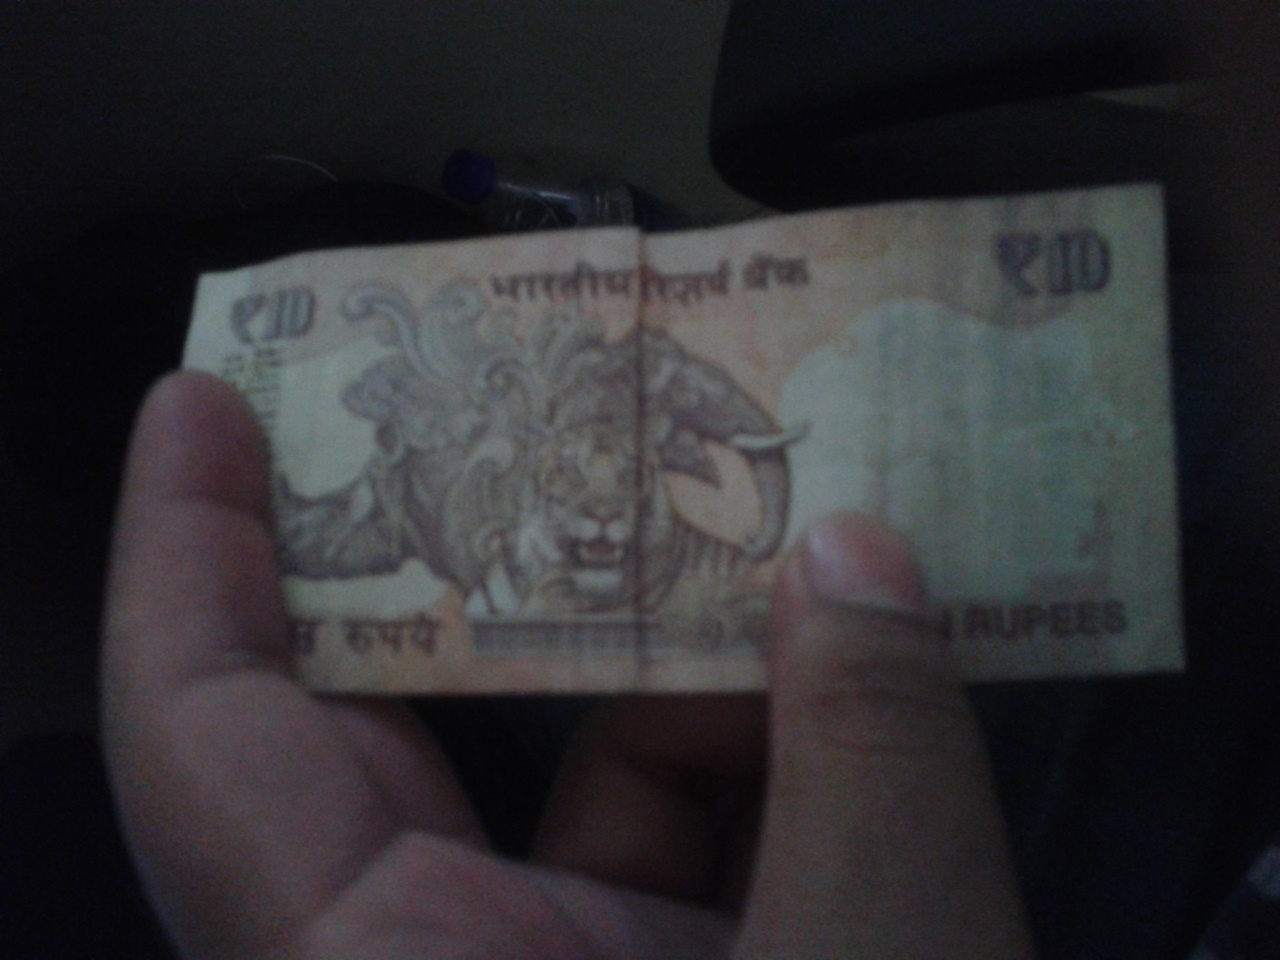
\includegraphics[width=60mm]{CHAPTERS/bd1.jpg}}
	\caption{Dataset of currency image taken in poor light condition}
\end{figure}
\noindent The above figure 3.10. shows the dataset of currency images taken in bad light condition so that if a person try to recognize the currency in poor light condition then the model will be able to determine the currency with high accuracy.\\
\begin{figure}[h!]
	\centering
	\includegraphics[]{}
	\subfigure[]{\label{fig:a}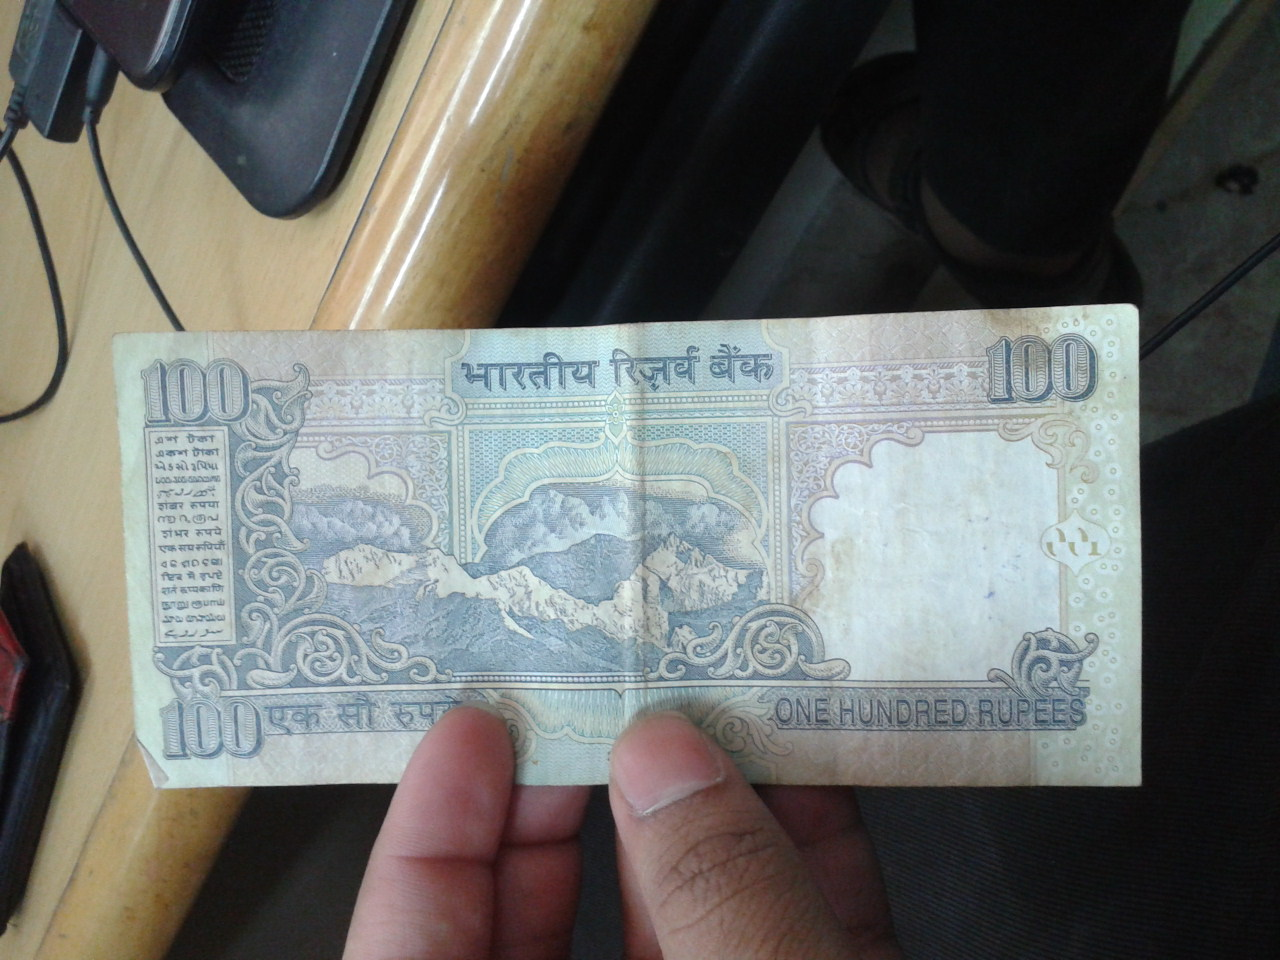
\includegraphics[width=60mm]{CHAPTERS/back1.jpg}}
	\subfigure[]{\label{fig:b}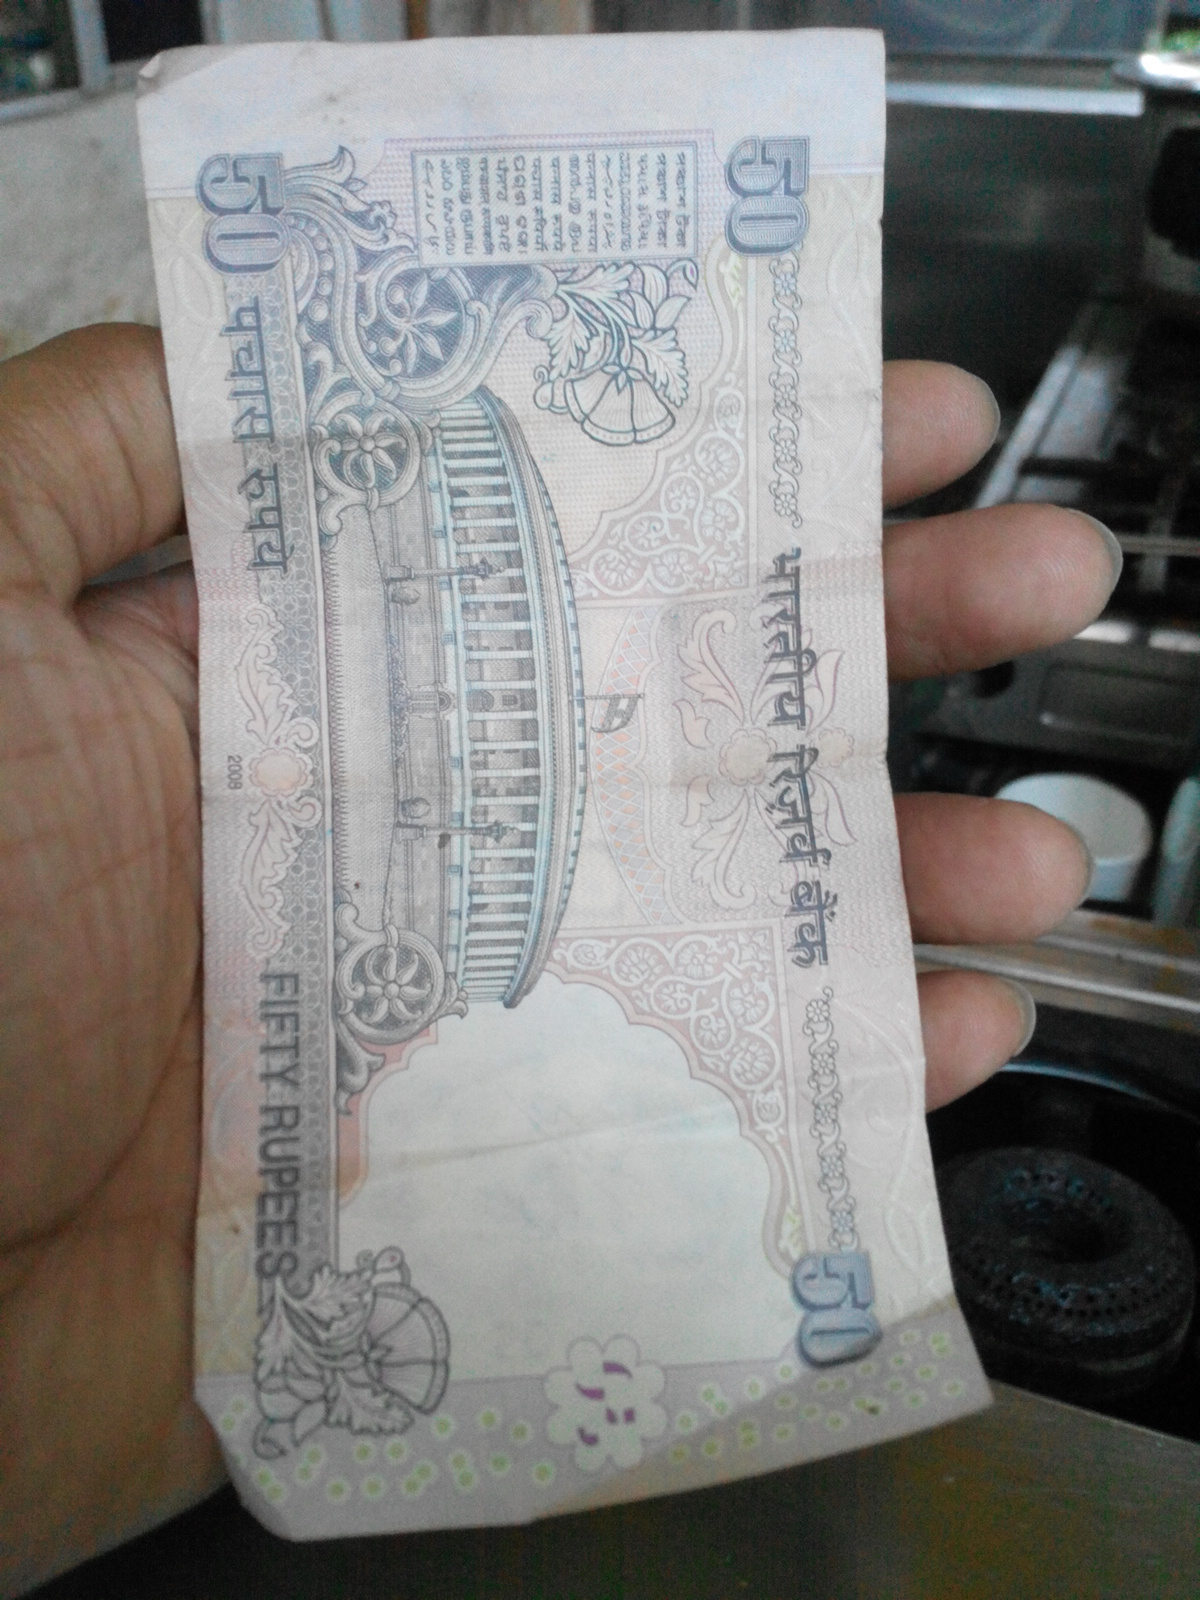
\includegraphics[width=40mm]{CHAPTERS/back2.jpg}}
	\caption{Dataset of currency image taken from back side of currency note}
\end{figure}\\
\noindent The above figure 3.11 shows the dataset of currency image taken from back side so that the CNN model is able to determine the currency from back side also.\\
\noindent Thus by taking the photo of the currency from all direction and in all condition the accuracy of the dataset will increase.\newpage
\noindent{\bf Training of Data}\\\\
The below Figure 3.12. (a), (b), (c) and (d) are the screenshots of training the model with different dataset.
\begin{figure}[h!]
	\centering
	\subfigure[]{\label{fig:a}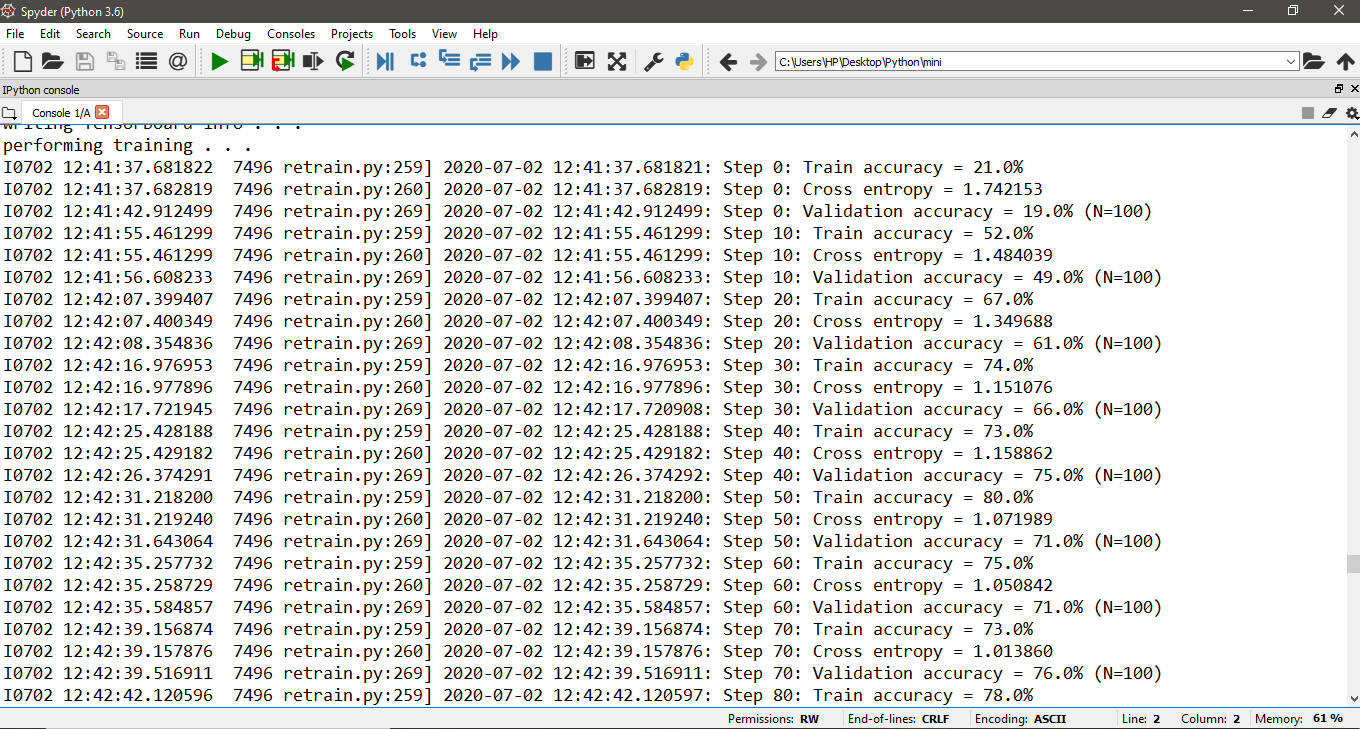
\includegraphics[width=70mm]{CHAPTERS/t1.PNG}}
	\subfigure[]{\label{fig:b}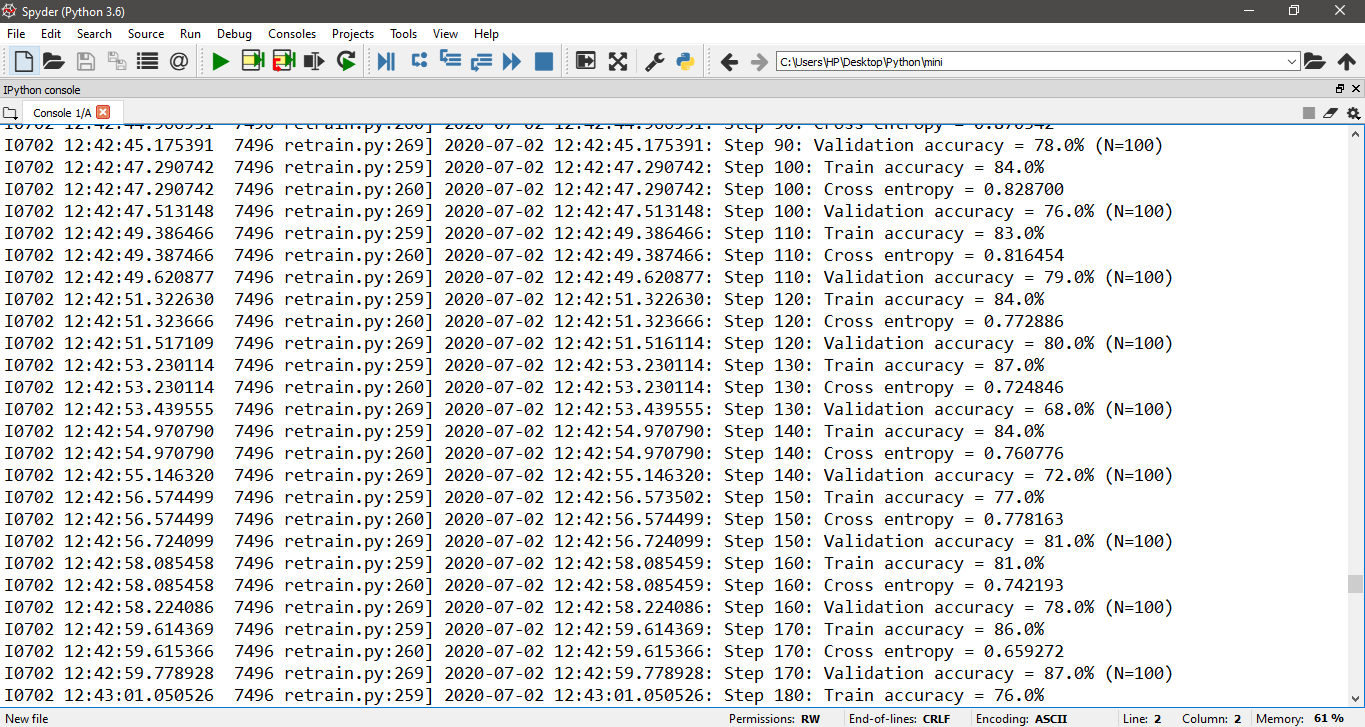
\includegraphics[width=70mm]{CHAPTERS/t2.PNG}}
	\subfigure[]{\label{fig:a}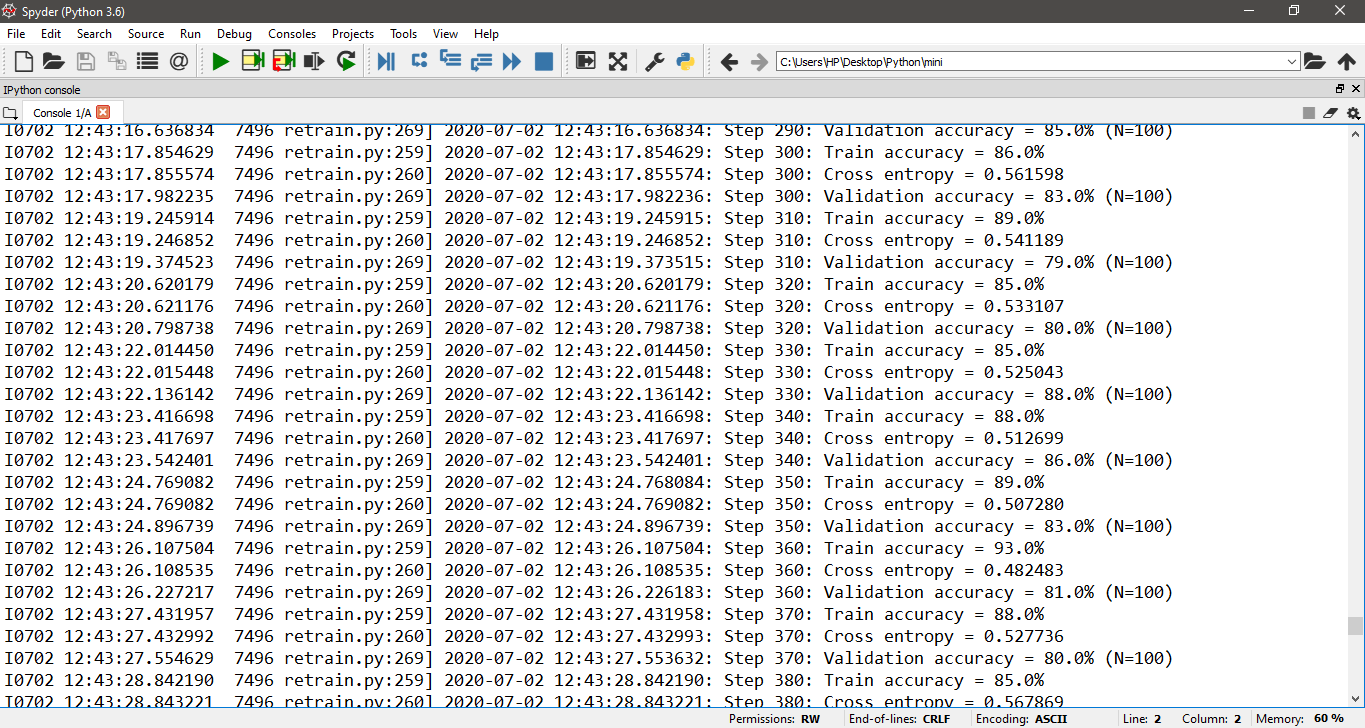
\includegraphics[width=70mm]{CHAPTERS/tt3.PNG}}
	\subfigure[]{\label{fig:b}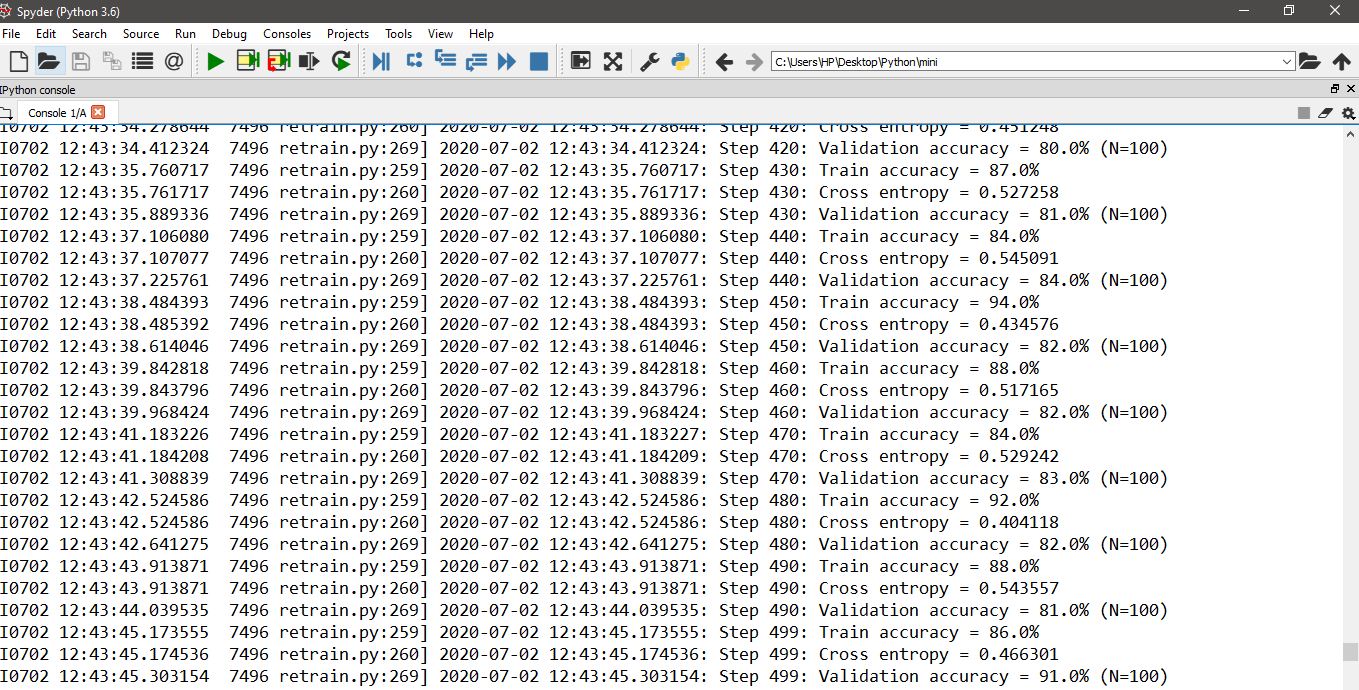
\includegraphics[width=70mm]{CHAPTERS/tt4.PNG}}
	\caption{Screenshot of training the CNN model }
\end{figure}

\newpage
\section{Flowchart}
\begin{figure}[h!]
    \centering
    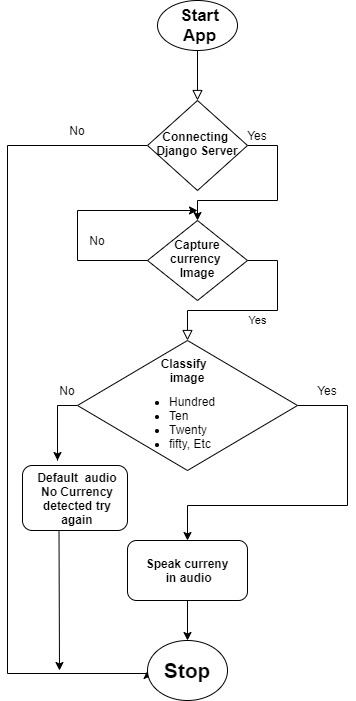
\includegraphics[width=0.5\textwidth]{CHAPTERS/f1.jpeg}
    \caption {Flow chart of currency detection}
\end{figure}
\noindent The above flowchart shown in Figure 3.13. represents the currency detection \noindent using camera of a device with the help of web \noindent app created by Django.
\newpage
\begin{itemize}
	\item First, It will try to connect with Django server and if successfully get connected then move to the next task else it will terminate their itself.
	\item Once the connection has been done it will capture the currency image and upload it to the Django server.
	\item Now, from the captured image it will try to classify the image from predefined dataset.
	\item Further, if it is able to classify the image then it will develop a text to speech algorithm and speaks the currency value in audio. 
	\item If it fails to classify the image then a default audio of no currency detected please try again will be given as output,
\end{itemize}
\section{Simulations}
\begin{figure}[h!]
	\centering
	\subfigure[]{\label{fig:a}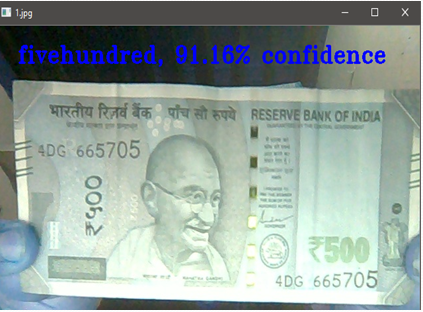
\includegraphics[width=65mm]{CHAPTERS/x2.PNG}}
	\subfigure[]{\label{fig:b}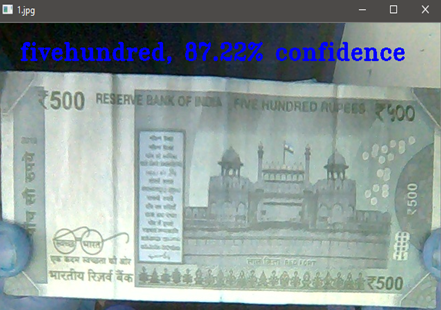
\includegraphics[width=65mm]{CHAPTERS/x3.PNG}}
	\subfigure[]{\label{fig:a}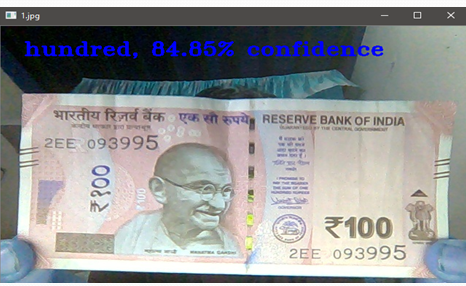
\includegraphics[width=65mm]{CHAPTERS/x9.PNG}}
	\subfigure[]{\label{fig:b}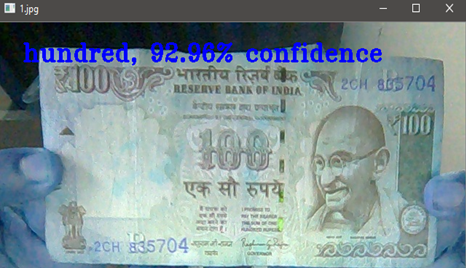
\includegraphics[width=65mm]{CHAPTERS/x4.PNG}}
	\caption{Result of image classification by the Neural Network for 500,100}
\end{figure}
\newpage
\noindent The above Figure 3.14. (a), (b), (c) and (d) are the simulations for different currency images with accuracy between 85-95 percent using the image clssification by neural network algorithm.\\
\begin{figure}
	\centering
	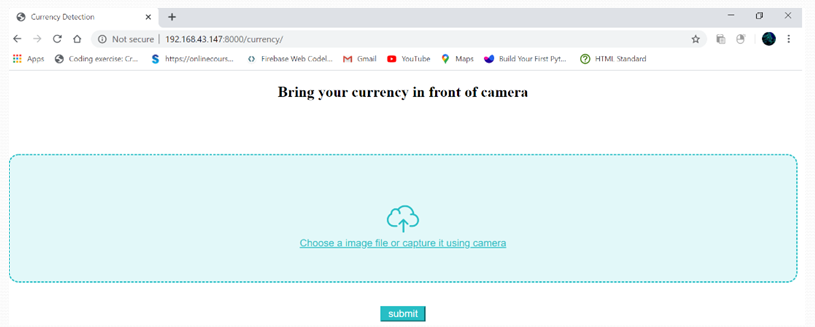
\includegraphics[width=0.9\textwidth]{CHAPTERS/x1.PNG}
	\caption{Django interface to capture currency image on browser}
\end{figure}
\begin{figure}
	\centering
	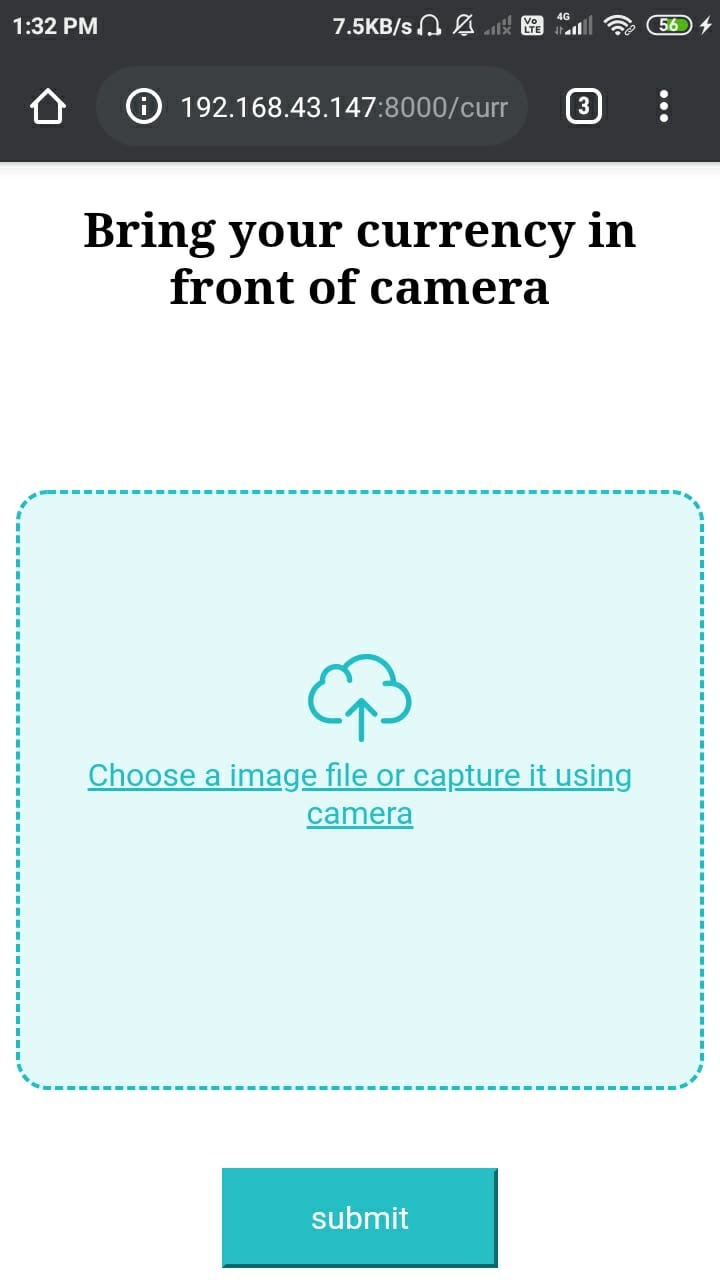
\includegraphics[width=0.3\textwidth]{CHAPTERS/I1.jpeg}
	\caption{Django interface to capture currency image on mobile phone}
\end{figure}
\begin{figure}[h!]
	\centering
	\subfigure[]{\label{fig:a}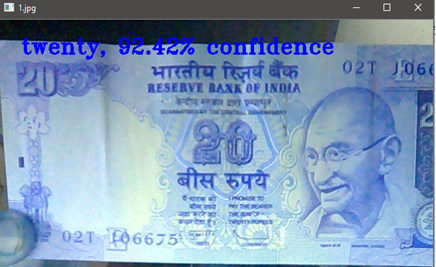
\includegraphics[width=65mm]{CHAPTERS/x6.PNG}}
	\subfigure[]{\label{fig:b}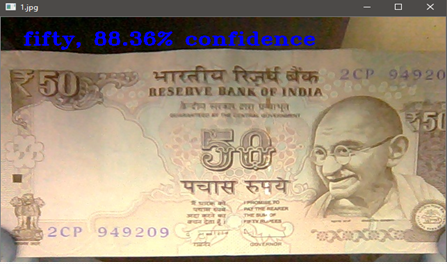
\includegraphics[width=65mm]{CHAPTERS/x7.PNG}}
	\subfigure[]{\label{fig:a}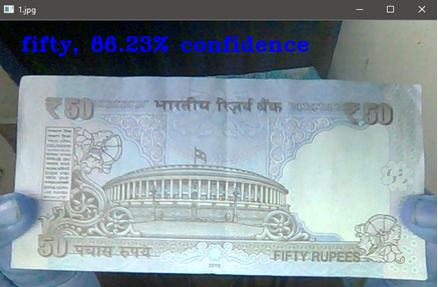
\includegraphics[width=65mm]{CHAPTERS/x8.PNG}}
	\subfigure[]{\label{fig:b}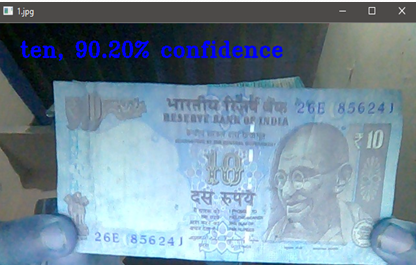
\includegraphics[width=65mm]{CHAPTERS/x5.PNG}}
	\caption{Result of image classification by the Neural Network for 20,50,10}
\end{figure}
\noindent The above figure 3.15. and Figure 3.16. shows the interface for currency detection web app developed using Django interface.
\begin{figure}
	\centering
	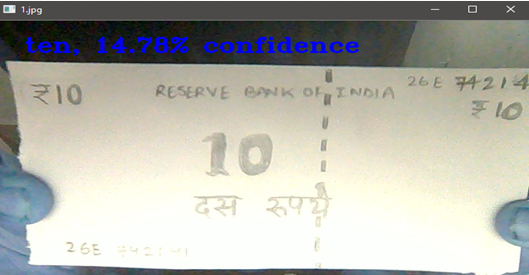
\includegraphics[width=0.6\textwidth]{CHAPTERS/x10.PNG}
	\caption{Result of accuracy for fake currency}
\end{figure}
\newpage
\noindent The above Figure 3.17. (a), (b), (c) and (d) are the simulation for accuracy of different currencies.\\
The accuracy of fake currency is shown below in Figure 3.16 here the threshold cut-off for accuracy is fixed at {\bf 75} percent  so if any accuracy of any currency come less than threshold cutoff  then the system will declare it as fake currency.
\chapter{MEDICINE DETECTION}
\section{Overview}
 As mentioned earlier about the medicine detection in the starting of this report where a blind persons and old age persons are facing difficulties in finding the name of the medicine.\\In this project camera of an device is used to get the input as image, where the input is a picture of medicine with the name of the medicine.\\These images can be manipulated using image processing and OpenCV tools in python.\\Once the pre-processed image is obtained then it will cropped and thresholded to get the accurate and better result from the image taken by the blind person and old age person.\\In the next stage it will extract the name of medicine from the cover of the medicine image taken by the user, then it will convert that text into speech using TTS technology.\\In Figure 4.1. an example of an medicine image is shown with the name \textbf{\textit{Hydrocotisone}} and other text written on its cover. Here in this project aim is to extract the name of medicine from all other informations. 
\begin{figure}
	\centering
	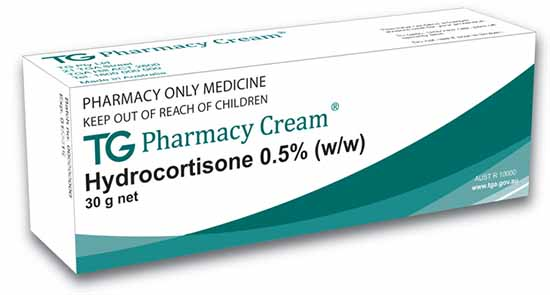
\includegraphics[width=70mm]{CHAPTERS/c31.PNG}
	\caption{Medicine image with name of the medicine}
\end{figure}
\newpage
\section{Block Diagram}
\noindent The Block Diagram of medicine detection is shown in Figure 4.2.
\begin{figure}[h!]
    \centering
    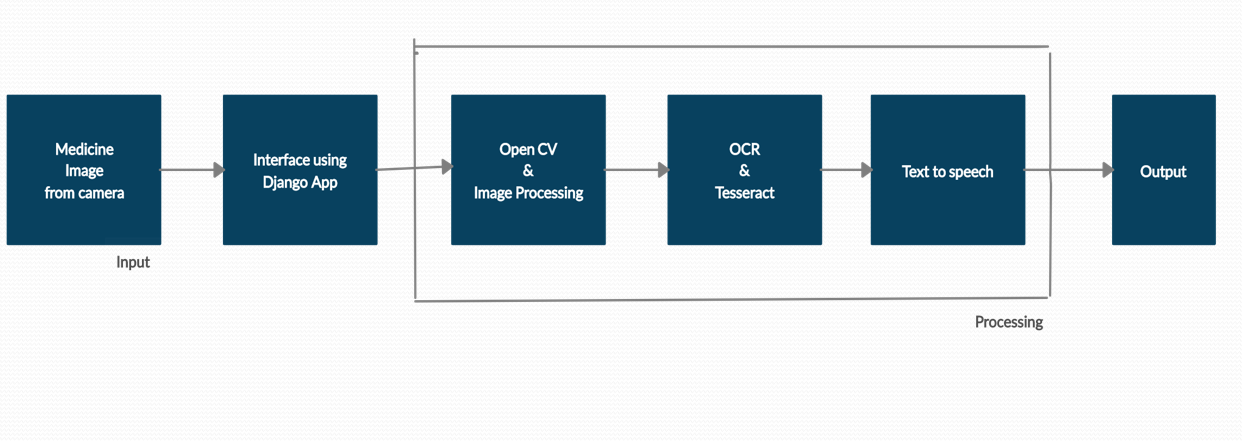
\includegraphics[width=1\textwidth]{CHAPTERS/c32.PNG}
    \caption{Block diagram of medicine detection}
\end{figure}
\section{Working}
First medicine image is taken from the camera of the device using Django interface and then saved it onto the Django server inside the test image folder by HTTPS POST method.\\Later, Image processing is used to extract the information on the image such as name of the medicine along with texts written on the image from the saved image inside the test image folder on Django server.\\Further, OpenCV tool in python is used to thresholding the image by converting RGB to Gray Scale, Color shifting, Cropping the ROI of an input image basically enhancement of the image to get accurate and proper results.\\OCR is used to recognize the the characters from the image and Tesseract is an engine which uses OCR techniques to identify the texts using AI.\citeauthor{9020104}
\newpage
\section{Algorithm}
\begin{itemize}
	\item It will match word by word in both the files, where file one is the where all the test extracted from the image of the medicine get stored and file two is the list of all the medicine names for the particular person for whom model is designed or trained.
	\item The word is matched in both the files using strip line method in python by using brute force algorithm ( nested for loop)
	\item The word that get matched is medicine name for which person has given the input as a image from camera of his/her phone. \citeauthor{9020103}
\end{itemize}
\section{Flowchart}
\begin{figure}[h!]
   \centering
    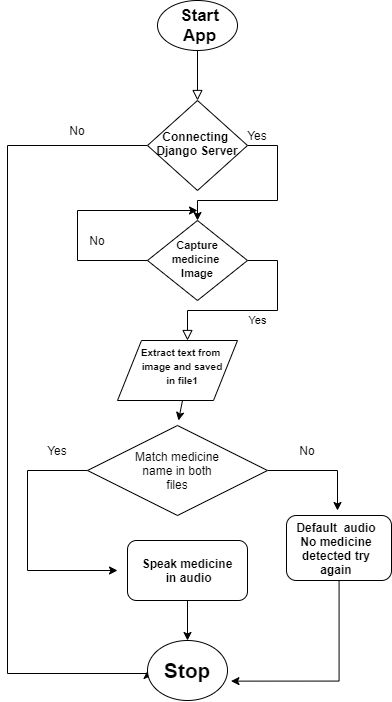
\includegraphics[width=0.5\textwidth]{CHAPTERS/c33.PNG}\\
    \caption {Flow chart of medicine detection}
\end{figure}
\newpage
\noindent The above flowchart shown in Figure 4.3. represents the medicine detection using
camera of a device with the help of web app created by Django. 
\begin{itemize}
	\item First, It will try to connect with Django server and if successfully get connected then move to the next task else it will terminate their itself.
	\item Once the connection has be done it will capture the medicine image and upload it to the Django server.
	\item Now, from the captured image it will extract the texts written on it and saved it into the txt file.
	\item Further, from the extracted texts information it will start matching the medicine name from both the txt files. If matches found name of the medicine is converted into speech using TTS technology or else a default audio of no medicine name detected will come from the speaker of the device.
	\item Finally after successful execution the process stop.
\end{itemize}
\section{Simulations}
\begin{figure}[h!]
	\centering
	\includegraphics[]{}
	\subfigure[]{\label{fig:a}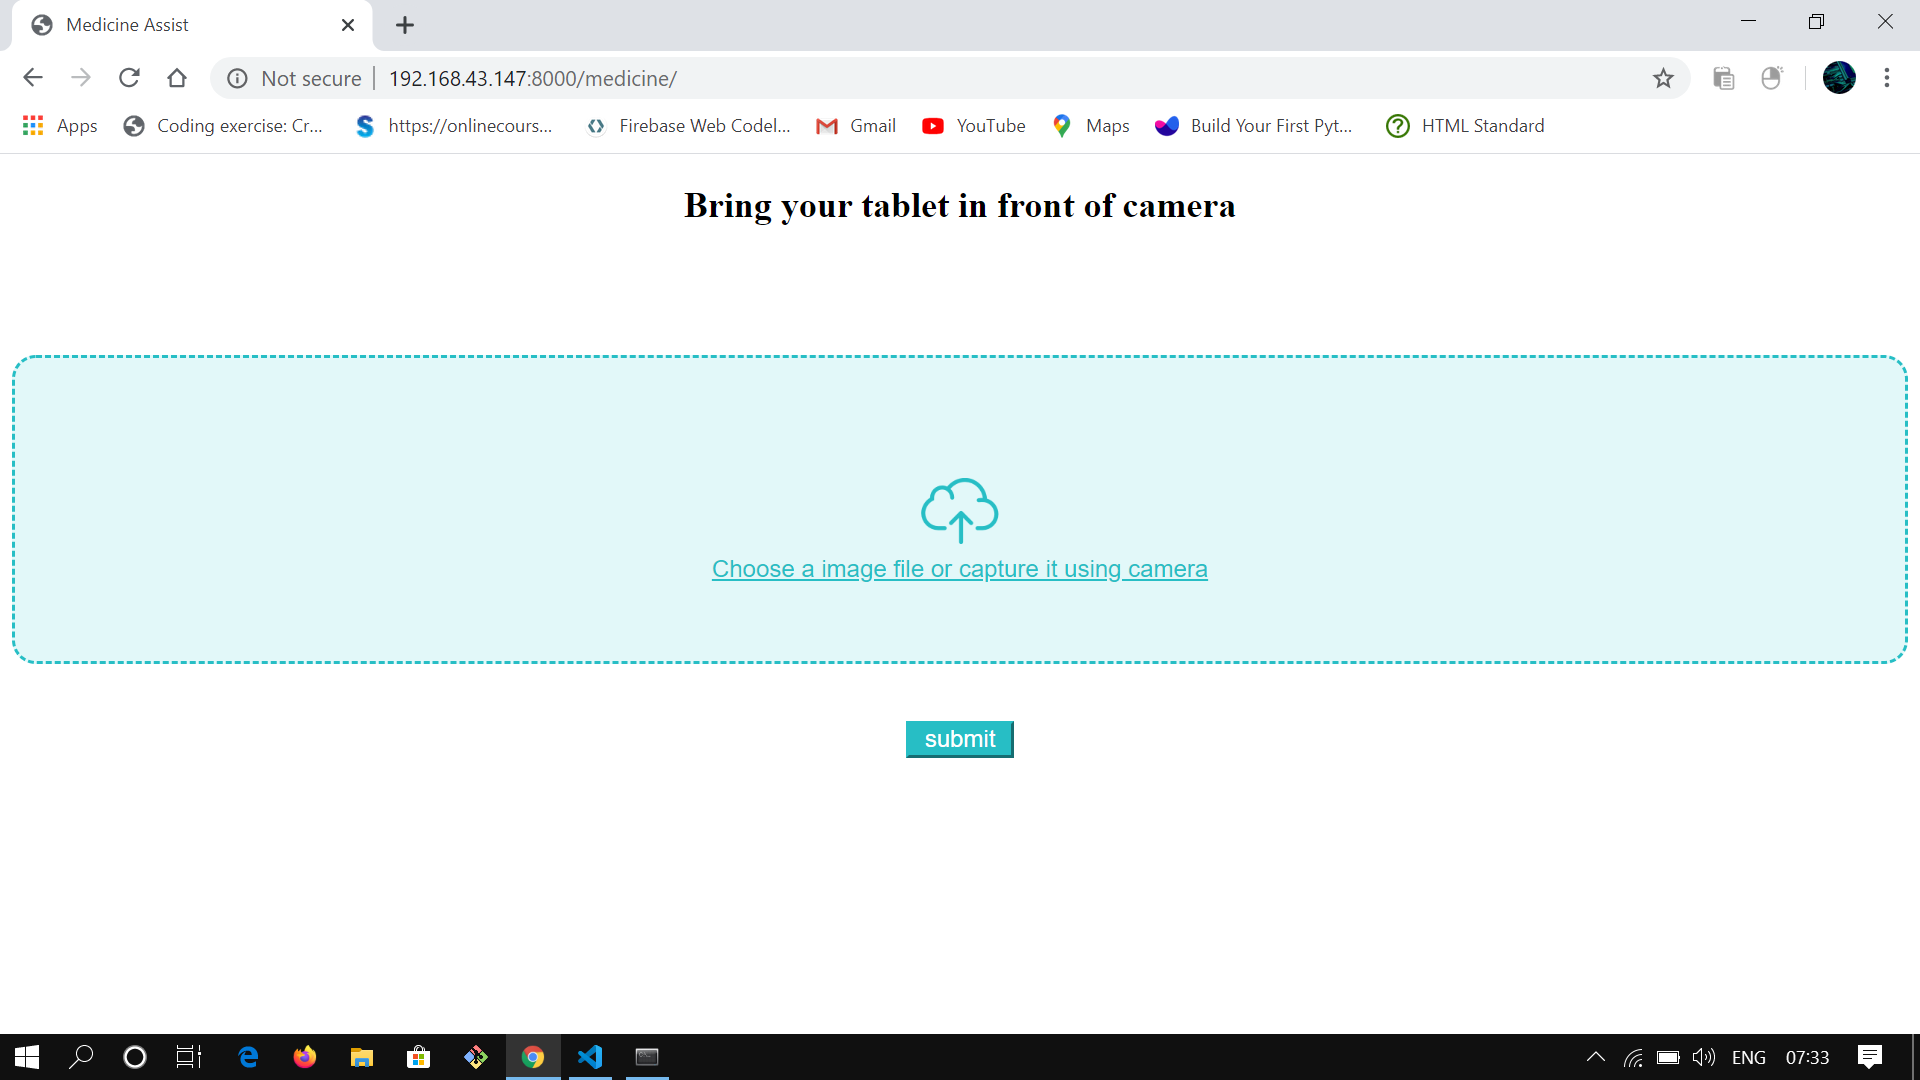
\includegraphics[width=120mm]{CHAPTERS/s1.png}}
	\subfigure[]{\label{fig:b}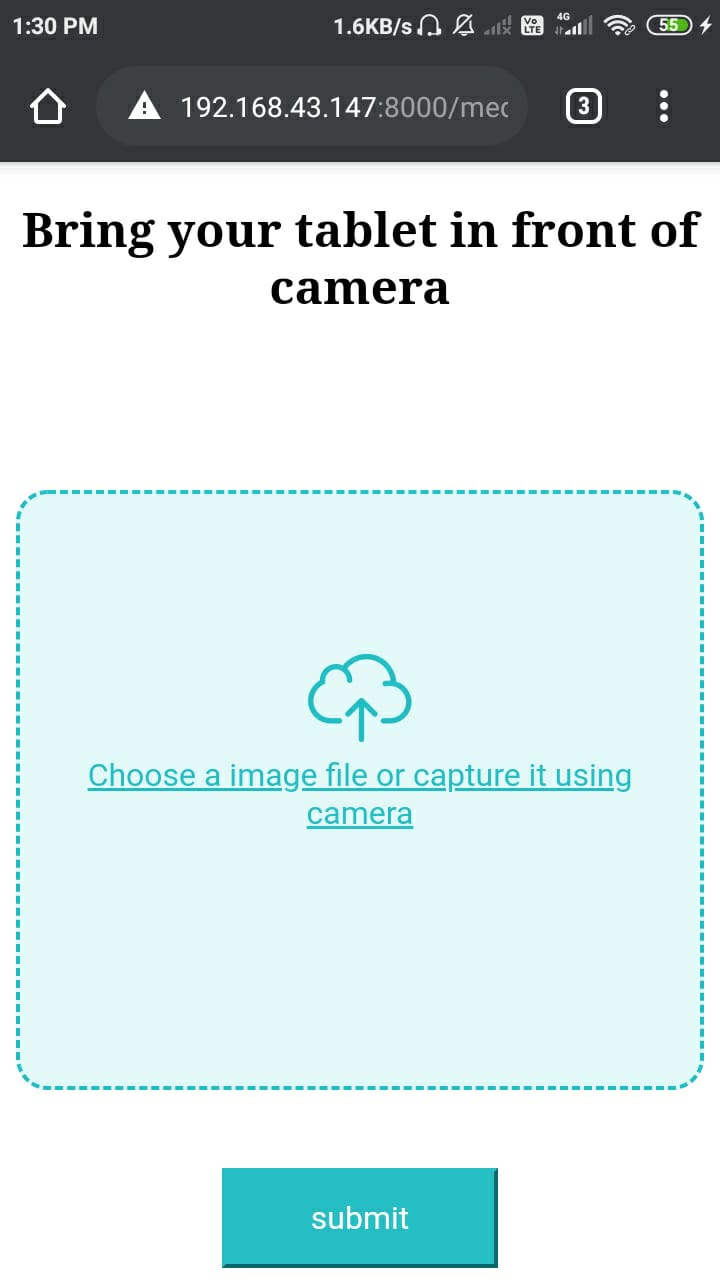
\includegraphics[width=35mm]{CHAPTERS/I2.jpeg}}
	\subfigure[]{\label{fig:c}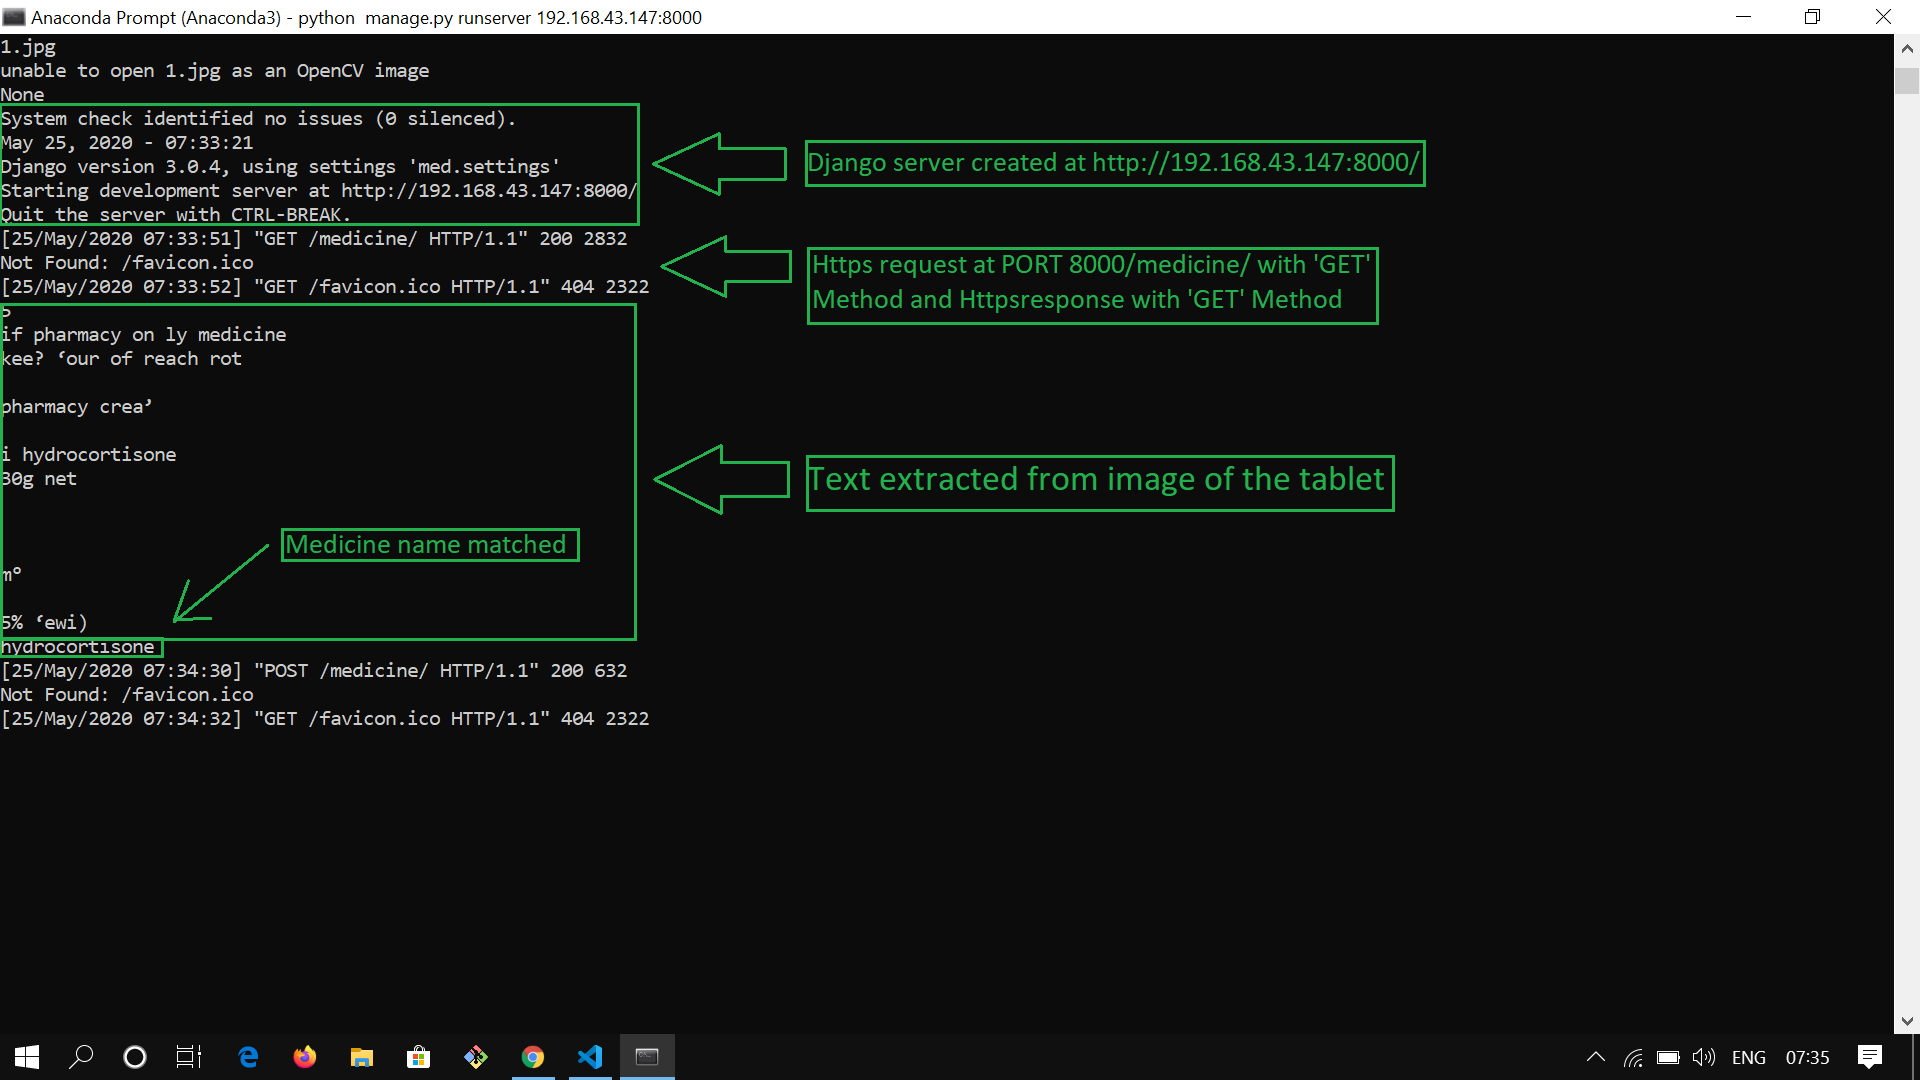
\includegraphics[width=110mm]{CHAPTERS/s2.png}}
	\caption{(a) and (b) Django interface to capture the medicine image on browser and mobile. (c) Anaconda prompt. }
\end{figure}
\noindent The below Figure 4.4. (a) and Figure 4.4. (b) is the interface for our web app created using basic HTML, CSS and JS code. The idea behind of making the blue box bigger as much as possible because when person will tap on it more likely he/she will touch that blue box. Blue box where blind person need to tap on it  to open the camera of the device to capture the image of the medicine for which he want to detect the name of the medicine with doses.\\Js code is written for the submit button if the blind person is not able to find the submit button it will automatically submit the capture image after fixed duration.
\\
\newpage

\noindent The above figure 4.4. (c) is the backend prompt view of medicine detection part of this project. First it will connect to the Django server by running python runserver command with the IP an port number. Once the server is connected it will acknowledge by HTTPS 'POST' and 'GET' method just to ensure the connection between interface and python source file.\\
\newpage
\noindent In the figure, inside the bigger green box the text is extracted from the medicine image which shown above in this report at figure 4.1. Once all the text get extracted from the the captured image then all of them is get converted into lowercase so that comparison is easy and less time consuming.\\Inside the lower small green box is the name of the medicine and according the name of the medicine it will return audio file containing name of the medicine and prescribed doses by the doctor to the Django interface so that blind person can listen the audio and took the medicine with his/her comfort.
\newpage
\chapter{RESULTS}
\noindent The {\bf EYE FOR BLIND} can help the blind person in detection of currency note and medicine name. By  this the blind person would take care of himself without the help of any care takers. This would make their life easier and simpler. The talkback feature used would help them to access the application easily without any complications.
\begin{itemize}
	\item This project would help blind person to detect the proper currency that they have received or which they need to to give without being cheated for receiving wrong currency or by avoiding giving wrong currency. This would make them economically stable and strong
	\item Not only in currency detection but also this project would help blind person to recognise the name of the tablet and also help them to know that how much  dosages they need to take as per the name of the tablet.
\end{itemize}
\noindent This project would help the blind persons both in economical way and in perspective of health. This would make their life easier and make them confident.\\\\ \textbf{\Large GitHub Repository of this project :} \href{https://github.com/mastersumant/mini_project}{\Large \color{blue} Eye for blind }.
\chapter{APPLICATIONS, ADVANTAGES and DISADVANTAGES}
\section{Applications}
\newline
\begin{itemize}
\item Blind persons will be able to recognise the correct
currency without getting cheated in any type of money transaction.

\item Blind persons always need not to be dependent on others to know which medicines they need to take a particular time. 
\end{itemize}
\section{Advantages}
\newline\begin{itemize}
\item This project will work on mobile phones only no need to buy any extra things. 
\item This work is implemented using TalkBack for android and Voiceover for iOS that means blind person can easily access the application. 
\item Easy to setup. 
\item Open source tools were used for this project.
\item Accessible to all the device irrespective of the OS. 
\item Cheap and cost efficient. 
\end{itemize}
\section{Disadvantages}
\newline
\begin{itemize}
\item It is very difficult to determine the currency as a fake one when it is an exact copy of the real currency.
\item For medicine part the image should be taken from any side where name of the medicine is written.
\end{itemize}
\newpage
\chapter{CONCLUSION AND FUTURE SCOPE}
\section{Conclusion}
\noindent This work shows how visually impaired person (blind person) can protect themselves by getting cheated in terms of money transaction and also how to reduce the dependency on other people to take right amount of medicine at right time\\Whenever the blind person takes the image using his phone camera the image will be compared with the data set which is created. After comparing the image if it gets the accuracy above the threshold value then it will gives the spoken feedback to the person by saying the value of the currency\\Similarly in case of medicine detection extract the name of the medicine and gives the spoken feedback as how many times that person need to take the medicine, thus making this work as one of the assistant for blind person.
\section{Future Scope}
\begin{itemize}\\
\\
\item Include the the data set of a photos that containing a persons images it can also be used to detect the person who have the blind person meets. 

\item It can also be used to to track the the blind person using GPS 

\end{itemize}



